% ===========================================================================
%  EPIC 2026 -- Fault-Tolerant Swarm Quadrotor Control for Non-Convex
%  Geodetic Mapping.  Slide deck, 20 min talk + 10 min Q&A.
%
%  Angka TIDAK pernah diketik di sini. \input{numbers} memuat file makro yang
%  SAMA dengan yang dipakai paper (docs/Full Paper - EPIC/generated/numbers.tex,
%  dihasilkan swarm_ws/analysis/skema5_paper_analysis.py). Makro yang tidak ada
%  menggagalkan kompilasi, persis seperti yang kita mau.
%
%  Bangun lewat Makefile, bukan pdflatex langsung -- TEXINPUTS perlu diset.
%     make            -> main.pdf   satu berkas untuk semua: disubmit, dibaca di
%                                   mana pun, DAN dipresentasikan lewat pdfpc
%                                   (video lewat tautan run:, catatan + hitung
%                                   mundur lewat metadata pdfpc)
%     make pptx       -> main.pptx  cadangan untuk laptop panitia
%
%  Kalau video tidak mau diputar di pdfpc, ganti satu baris di bawah ke
%  \def\videomode{movie} dan bangun ulang: itu memakai anotasi /Movie dari
%  paket multimedia alih-alih tautan run:.
%
%  Gaya: judul frame adalah KLAIM, bukan topik. Bullet maksimal empat, pendek.
%  Uraian panjang masuk ke \note, bukan ke layar.
% ===========================================================================
\documentclass[aspectratio=169,11pt,t]{beamer}
\usepackage[T1]{fontenc}
% Tiga genre dari satu superfamily Source (lihat epicbeamer.sty): serif untuk
% judul, sans untuk isi, mono untuk besaran bernilai. Urutannya penting --
% sourcesanspro[default] yang terakhir supaya isi memakai sans.
\usepackage{sourceserifpro}
\usepackage{sourcecodepro}
\usepackage[default]{sourcesanspro}
\usepackage{newtxsf}
\usepackage{epicbeamer}

% Catatan pembicara + hitung mundur ditanam sebagai METADATA di main.pdf.
% pdfpc membacanya; pembaca PDF biasa tidak menampilkannya sama sekali, jadi
% berkas yang disubmit tetap bersih. Opsi "overridenote" membuat \note{} bawaan
% Beamer langsung menjadi catatan pdfpc -- tidak ada perintah baru untuk dihafal.
% ===========================================================================
%  Diagram TikZ untuk rantai penurunan.
%
%  Ditulis untuk audiens yang bukan orang kendali: tiap gambar menerjemahkan
%  SATU persamaan jadi sesuatu yang bisa ditunjuk. Warna mengikuti palet tema
%  (epicbeamer.sty), jadi tidak ada warna baru diperkenalkan di sini.
%
%    \diagfbd     Langkah 1  gaya menyamping hanya dari thrust yang dimiringkan
%    \diagbudget  Langkah 5  dead time + pengereman harus muat di clearance h
%    \diagrow     Langkah 7  hanya komponen MENDEKAT yang dibatasi
%    \diagarch    slide judul  tiga lapis + plant, satu kolom
% ===========================================================================
\usetikzlibrary{arrows.meta, angles, quotes, decorations.pathreplacing, calc}

\tikzset{
  vec/.style    = {-{Stealth[length=2.2mm]}, line width=0.8pt},
  vecfat/.style = {-{Stealth[length=2.8mm]}, line width=1.3pt},
  hair/.style   = {line width=0.4pt},
  lbl/.style    = {font=\scriptsize, inner sep=1.5pt},
  wee/.style    = {font=\tiny, inner sep=1.5pt},
}

% --------------------------------------------------------------- Langkah 1
% Kenapa miring adalah SATU-SATUNYA cara bergerak menyamping.
\newcommand{\diagfbd}{%
\begin{tikzpicture}[x=1cm, y=1cm]
  \def\th{26}\def\L{2.55}
  \pgfmathsetmacro{\tx}{\L*sin(\th)}
  \pgfmathsetmacro{\ty}{\L*cos(\th)}

  \draw[hair, epicpeach, dashed] (0,-1.5) -- (0,3.0);

  % badan quadrotor, dimiringkan \th
  \begin{scope}[rotate=-\th]
    \draw[line width=1.8pt, epicbrick] (-1.0,0) -- (1.0,0);
    \draw[epicclay, line width=1.0pt] (-1.32,0.14) -- (-0.68,0.14);
    \draw[epicclay, line width=1.0pt] ( 0.68,0.14) -- ( 1.32,0.14);
    \fill[epicbrick] (-1.0,0) circle (1.7pt) (1.0,0) circle (1.7pt);
  \end{scope}

  % thrust tegak lurus badan
  \draw[vecfat, epicrust] (0,0) -- (\tx,\ty)
        node[lbl, epicrust, anchor=south west, inner sep=2pt] {$T$};

  % penguraian: dua kaki persegi panjang
  \draw[hair, epicpeach] (\tx,\ty) -- (0,\ty);
  \draw[hair, epicpeach] (\tx,\ty) -- (\tx,0);
  \draw[vec, epicclay] (0,0) -- (0,\ty)
        node[lbl, epicclay, anchor=east, pos=0.68] {$T\cos\theta$};
  \draw[vec, epicclay] (0,\ty) -- (\tx,\ty)
        node[lbl, epicclay, anchor=south, pos=0.5] {$T\sin\theta$};

  \draw[vec, epicbrick] (0,0) -- (0,-1.25)
        node[lbl, epicbrick, anchor=north] {$mg$};

  \coordinate (O) at (0,0);
  \coordinate (V) at (0,0.95);
  \coordinate (B) at ({0.95*sin(\th)},{0.95*cos(\th)});
  % Urutan titik penting: pic 'angle' menyapu BERLAWANAN arah jarum jam, jadi
  % V--O--B akan menggambar 334 derajat (nyaris lingkaran penuh), bukan 26.
  \pic[draw=epicrust, line width=0.6pt, angle radius=8mm,
       "{$\theta$}"{epicrust, font=\scriptsize, inner sep=1pt}] {angle = B--O--V};

  \node[wee, epicclay, anchor=south] at (0,3.0) {vertical};
\end{tikzpicture}}

% --------------------------------------------------------------- Langkah 5
% Anggaran jarak: dead time + pengereman harus muat di dalam clearance h.
\newcommand{\diagbudget}{%
\begin{tikzpicture}[x=1cm, y=1cm]
  \def\Hh{8.0}\def\Td{2.3}

  \fill[epicpeach] (\Hh+0.8,0) circle (0.78);
  \draw[epicclay, line width=0.8pt] (\Hh+0.8,0) circle (0.78);
  \node[wee, epicbrick] at (\Hh+0.8,0) {obstacle};

  % drone
  \draw[line width=1.8pt, epicbrick] (-0.5,0) -- (0.5,0);
  \draw[epicclay, line width=1.0pt] (-0.68,0.13) -- (-0.32,0.13);
  \draw[epicclay, line width=1.0pt] ( 0.32,0.13) -- ( 0.68,0.13);
  \fill[epicbrick] (-0.5,0) circle (1.7pt) (0.5,0) circle (1.7pt);
  \draw[vec, epicrust] (0.85,0) -- (1.85,0)
        node[lbl, epicrust, anchor=south, pos=0.5] {speed $s$};

  % clearance
  \draw[hair, epicclay] (0,-0.9) -- (0,-1.85);
  \draw[hair, epicclay] (\Hh,-0.9) -- (\Hh,-1.85);
  \draw[{Stealth[length=2mm]}-{Stealth[length=2mm]}, epicclay, line width=0.7pt]
        (0,-1.6) -- (\Hh,-1.6);
  \node[lbl, epicclay, fill=white, inner sep=2pt] at (\Hh/2,-1.6)
    {clearance $h$ to the surface};

  % dua ruas anggaran
  \draw[decorate, decoration={brace, amplitude=5pt}, epicrust, line width=0.8pt]
        (0,1.0) -- (\Td,1.0)
        node[midway, lbl, epicrust, anchor=south, yshift=4pt] {$s\,T_d$};
  \draw[decorate, decoration={brace, amplitude=5pt}, epicbrick, line width=0.8pt]
        (\Td,1.0) -- (\Hh,1.0)
        node[midway, lbl, epicbrick, anchor=south, yshift=4pt]
        {$D(s)$, the braking distance};
  \draw[hair, epicpeach, dashed] (\Td,-0.9) -- (\Td,1.0);

  \node[wee, epicrust, anchor=north, align=center] at (\Td/2,-0.35)
    {reacting:\\[-0.3ex] still closing};
  \node[wee, epicbrick, anchor=north] at ({(\Td+\Hh)/2},-0.35) {slowing down};
\end{tikzpicture}}

% --------------------------------------------------------------- Langkah 7
% Satu baris constraint: hanya komponen MENDEKAT yang dibatasi.
\newcommand{\diagrow}{%
\begin{tikzpicture}[x=1cm, y=1cm]
  \fill[epicpeach] (5.3,0) circle (0.8);
  \draw[epicclay, line width=0.8pt] (5.3,0) circle (0.8);
  \node[wee, epicbrick] at (5.3,0) {hazard};

  \fill[epicbrick] (0,0) circle (2.4pt);
  \node[wee, epicbrick, anchor=north east] at (-0.1,-0.12) {agent};

  \draw[hair, epicpeach, dashed] (0,0) -- (4.5,0);
  \draw[vec, epicclay] (0,0) -- (1.35,0);
  \node[lbl, epicclay, anchor=south] at (0.7,0.06) {$\mathbf{n}_{ij}$};

  % kecepatan yang diminta, dan penguraiannya
  \draw[vecfat, epicrust] (0,0) -- (3.0,1.9)
        node[lbl, epicrust, anchor=south west] {$\mathbf{u}_i$};
  \draw[hair, epicbrick, dashed] (3.0,1.9) -- (3.0,0);
  \draw[hair, epicbrick, dashed] (3.0,1.9) -- (0,1.9);
  \draw[vec, epicbrick] (0,0) -- (3.0,0);
  \node[wee, epicbrick, anchor=north] at (2.2,-0.12) {closing component};
  \draw[vec, epicbrick] (0,0) -- (0,1.9);
  \node[wee, epicbrick, anchor=south, rotate=90] at (-0.16,0.95) {tangential};

  % batas
  \draw[epicrust, line width=1.1pt, dash pattern=on 2.5pt off 2pt]
        (3.6,-0.95) -- (3.6,2.5);
  \node[lbl, epicrust, anchor=south, align=center] at (3.6,2.5)
    {capped at $\lambda_{ij}\varphi(h_{ij})$};
  \node[wee, epicclay, anchor=north, align=center] at (2.4,-1.05)
    {only the closing component is capped --- turning is free};
\end{tikzpicture}}

% --------------------------------------------------- kontrak masuk/keluar
% Strip tiga kotak: APA YANG MASUK (dengan satuan) -> APA YANG DIHITUNG ->
% APA YANG KELUAR (dengan satuan). Dipakai sekali di tiap lapis, sehingga
% keluaran satu lapis terlihat persis menjadi masukan lapis berikutnya.
\newcommand{\iobox}[4]{% #1 x  #2 judul  #3 warna judul  #4 isi
  \node[draw=epicboxline, line width=0.5pt, fill=white, rounded corners=1pt,
        minimum width=38mm, minimum height=21mm, align=left, inner sep=2.2mm,
        font=\scriptsize, text=epicbrick, anchor=north west] (b#1) at (#1,0) {#4};
  \node[fill=#3, text=white, font=\bfseries\tiny, inner xsep=2mm, inner ysep=0.9mm,
        anchor=north west] at ($(b#1.north west)+(1.6mm,1.9mm)$) {#2};}

\newcommand{\diagio}[3]{%
\begin{tikzpicture}[x=1mm, y=1mm]
  \iobox{0}{WHAT GOES IN}{epicclay}{#1}
  \iobox{45}{WHAT IS COMPUTED}{epicrust}{#2}
  \iobox{90}{WHAT COMES OUT}{epicbrick}{#3}
  \draw[vec, epicclay] (38.5,-9.5) -- (44,-9.5);
  \draw[vec, epicclay] (83.5,-9.5) -- (89,-9.5);
\end{tikzpicture}}

% ------------------------------------------- kaskade low level + satuannya
% Rantai yang benar-benar dieksekusi 250 kali per detik, dengan SATUAN di tiap
% panah -- itu yang membuat jelas apa yang masuk dan apa yang keluar.
\newcommand{\diagcascade}{%
\begin{tikzpicture}[x=1mm, y=1mm,
   blk/.style={draw=epicrust, line width=0.6pt, fill=epicbeige!35, rounded corners=1pt,
               minimum width=20mm, minimum height=10mm, align=center,
               font=\tiny, text=epicbrick},
   sig/.style={font=\tiny, text=epicclay, inner sep=1pt}]
  \node[blk] (pf) at (0,0)   {pre-filter};
  \node[blk] (op) at (28,0)  {outer PID};
  \node[blk] (ip) at (56,0)  {inner PD};
  \node[blk] (mx) at (84,0)  {mixer};
  \node[draw=epicclay, line width=0.7pt, fill=epicpeach!40, rounded corners=1pt,
        minimum width=20mm, minimum height=10mm, align=center, font=\tiny,
        text=epicbrick] (pl) at (112,0) {quadrotor};

  % jalur maju; label SINYAL di atas panah, bukan di atas kotak
  \draw[vec, epicbrick] (-17,0) -- (pf);
  \node[sig, anchor=south] at (-8.5,6) {$\mathbf{p}^\star$ [m]};
  \node[sig, anchor=north, text=epicrust] at (-8.5,-6) {from mid level};
  \foreach \a/\b/\x/\t in {pf/op/14/{[m], [m/s]}, op/ip/42/{$\theta_{\mathrm{ref}}$ [rad]},
                           ip/mx/70/{$\tau$ [N$\cdot$m]}, mx/pl/98/{$\Omega$ [rad/s]}} {
    \draw[vec, epicbrick] (\a) -- (\b);
    \node[sig, anchor=south] at (\x,6) {\t};}

  % umpan balik: dua lintasan terpisah dari plant
  \draw[vec, epicclay] (pl.south) -- (112,-13) -- (56,-13) -- (ip.south);
  \node[sig, anchor=south] at (84,-12.6) {$\theta,\dot\theta$ [rad], [rad/s]};
  \draw[vec, epicclay] (116,-5) -- (116,-22) -- (28,-22) -- (op.south);
  \draw[epicclay, line width=0.8pt] (pl.south east) ++(-2,0) -- (116,-5);
  \node[sig, anchor=south] at (72,-21.6) {$\mathbf{p},\mathbf{v}$ [m], [m/s]};

  \node[sig, text=epicrust, anchor=north west, align=left] at (-17,-26)
    {the whole chain runs 250 times per second};
\end{tikzpicture}}

% ------------------------------------------------- arsitektur, slide judul
% Gambaran tiga lapis dalam satu kolom: tiap panah ke bawah adalah keluaran
% satu lapis yang menjadi masukan lapis di bawahnya; satu panah balik membawa
% odometri + LiDAR dari simulator ke ketiga lapis.
\newcommand{\diagarch}{%
\begin{tikzpicture}[x=1mm, y=1mm,
   lay/.style={draw=epicboxline, line width=0.5pt, fill=epicboxfill,
               rounded corners=1pt, minimum width=46mm, minimum height=6.4mm,
               align=left, inner xsep=2mm, inner ysep=1.4mm, font=\tiny, text=epicbrick,
               text width=42mm},
   tag/.style={font=\bfseries\tiny, text=white, inner xsep=1.3mm,
               inner ysep=0.6mm, anchor=south west},
   sig/.style={font=\tiny, text=epicclay, inner sep=1pt, anchor=west}]
  \node[lay] (hi) at (0,0)   {Voronoi cells $\to$ boustrophedon lanes\\
                              re-partition when an agent dies};
  \node[lay] (mi) at (0,-12) {CBF-QP safety filter\\
                              obstacles, walls, neighbours};
  \node[lay] (lo) at (0,-24) {\cL{PID-LQR} \textbar{} \cH{PID-$H_\infty$}\\
                              position $\to$ four rotor speeds};
  \node[lay, draw=epicclay, fill=epicpeach!40] (pl) at (0,-36)
       {Gazebo \textperiodcentered{} 7 quadrotors\\
        wind \textperiodcentered{} cylinders \textperiodcentered{} agent loss};
  \foreach \n/\t/\c in {hi/HIGH \textperiodcentered{} event/epicclay,
                        mi/MID \textperiodcentered{} 20 Hz/epicrust,
                        lo/LOW \textperiodcentered{} 250 Hz/epicbrick,
                        pl/PLANT/epicclay}
    \node[tag, fill=\c] at ($(\n.north west)+(1.6mm,-0.9mm)$) {\t};
  \foreach \a/\b/\t in {hi/mi/lane, mi/lo/safe velocity, lo/pl/rotor speeds} {
    \draw[vec, epicbrick] (\a.south) -- (\b.north);
    \node[sig] at ($(\a.south)!0.5!(\b.north)+(1mm,0)$) {\t};}
  % umpan balik ke ketiga lapis
  \draw[vec, epicclay] (pl.east) -- ++(3,0) coordinate (fb) |- (hi.east);
  \foreach \n in {mi,lo} \draw[vec, epicclay] (fb |- \n.east) -- (\n.east);
  \node[font=\tiny, text=epicclay, rotate=90, anchor=north] at ($(fb)+(0.4,18)$)
       {odometry \textperiodcentered{} LiDAR};
\end{tikzpicture}}
         % diagram TikZ untuk rantai penurunan
\usepackage[overridenote]{pdfpc}
\pdfpcsetup{duration=27, lastminutes=3}

\def\videomode{link}      % link | movie  (lihat catatan di atas)
\input{numbers}           % <-- file yang sama dengan paper
% DIHASILKAN OTOMATIS oleh tools/build_media.py -- JANGAN DIEDIT.
\newcommand{\SlowHthree}{5.4}
\newcommand{\SlowHfour}{4.1}
\newcommand{\SlowHfive}{3.9}
       % <-- faktor gerak lambat, dari tools/build_media.py
\renewcommand{\sectioncount}{9}

\title{Fault-Tolerant Swarm Quadrotor Control for Non-Convex Geodetic Mapping}
\author{Izma Alhazmi Herdian}
\date{24 October 2026}
\hypersetup{pdftitle={\inserttitle}, pdfauthor={Izma Alhazmi Herdian},
            colorlinks=false, pdfborder={0 0 0}}

\begin{document}

% =============================================== 0. Pembuka (1,0 min) ======
{\setbeamertemplate{headline}{}\setbeamertemplate{footline}{}
\begin{frame}[plain]
  \mins{3}%
  \begin{tikzpicture}[remember picture,overlay]
    \fill[epicbrick] (current page.north west) rectangle
      ([yshift=-27mm]current page.north east);
    \fill[epicclay] ([yshift=-27mm]current page.north west) rectangle
      ([yshift=-27.9mm]current page.north east);
    % arsitektur di kolom kanan, di bawah pita judul
    \node[anchor=north east, inner sep=0pt]
      at ([xshift=-6mm, yshift=-34mm]current page.north east) {\scalebox{0.86}{\diagarch}};
  \end{tikzpicture}%
  \vskip4mm
  \begin{minipage}{0.92\linewidth}
    {\color{epicwhite}\headfont\fontsize{19}{23}\selectfont
     Fault-Tolerant Swarm Quadrotor Control\\for Non-Convex Geodetic Mapping\par}
  \end{minipage}
  \vskip16mm
  {\color{epicrust}\headfont\small
   Izma Alhazmi Herdian\textsuperscript{1,2}\quad
   Sulthan Naufal Affan\textsuperscript{1}\\[0.6ex]
   Estiyanti Ekawati\textsuperscript{1,2}\quad
   Faqihza Mukhlish\textsuperscript{1,2}\par}
  \vskip2.5mm
  {\color{epicbody}\small
   \textsuperscript{1}Engineering Physics Department, Institut Teknologi Bandung\\
   \textsuperscript{2}Center for Instrumentation Technology and Automation, ITB\par}
  \vskip6mm
  {\color{epicmuted}\small
   5th Engineering Physics International Conference (EPIC 2026)\\
   24 October 2026 \textperiodcentered{} Bandar Lampung, Indonesia\par}
  \vfill
  {\color{epicrule}\rule{\linewidth}{0.4pt}\par}
  \vskip1.5mm
  {\color{epicclay}\bfseries\small github.com/izmaherdian/swarm-quadrotor-mapping\par}
  \narasi{Hello everyone. I am Izma Alhazmi Herdian, from Institut Teknologi Bandung. Today I present fault-tolerant swarm quadrotor control for mapping non-convex areas. On the right is the whole system in one picture: three control layers on top of a simulated swarm.}
    {Halo semuanya. Saya Izma Alhazmi Herdian, dari Institut Teknologi Bandung. Hari ini saya mempresentasikan kendali swarm quadrotor yang toleran terhadap kegagalan untuk memetakan area non-konveks. Di sebelah kanan adalah keseluruhan sistem dalam satu gambar: tiga lapis kendali di atas swarm yang disimulasikan.}
    {20 min + 10 min Q\&A. Open by naming the result out loud, then move on.
        Everything after this explains how --- and what failed.}
\end{frame}}

\kick{Opening}{}
\begin{frame}{Seven quadrotors, four regions, every stressor at once}
  \mins{4}%
  \centering
  \videoposter{overview_4regions}{0.70\textwidth}
  \figcaption{\hinf{} on rect, L, U and plus \textperiodcentered{} 8$\times$
    faster than mission time \textperiodcentered{} Gazebo left, RViz map right
    \textperiodcentered{} \videonote}
  \narasi{Before any equations, this is what the system does. Seven quadrotors split a region into cells, sweep their cells lane by lane, and steer around cylinders they discover with LiDAR, all under strong wind. In each of these four missions, two drones are killed in flight, and the survivors take over their work. Everything after this explains how.}
    {Sebelum masuk ke persamaan, inilah yang dilakukan sistemnya. Tujuh quadrotor membagi area menjadi sel, menyapu selnya lajur demi lajur, dan menghindari silinder yang mereka temukan dengan LiDAR, semuanya di bawah angin kencang. Di keempat misi ini, dua drone dimatikan saat terbang, dan drone yang tersisa mengambil alih pekerjaannya. Seluruh sisa presentasi menjelaskan bagaimana caranya.}
    {25 s. Let the clip run and say only what they are looking at: seven
        drones split the region, sweep lanes, avoid the cylinders, and two of
        them are killed mid-mission. Everything after this explains how.}
\end{frame}

\begin{frame}{Seven of eight missions finished after losing 28.6\% of the fleet}
  \mins{5}%
  \begin{itemize}\bulletgap
    \item The problem --- non-convex area, wind, unmapped obstacles, agent loss
    \item Three layers --- who sweeps where, a safety filter, two controllers
    \item Eight recorded missions, including the one that crashed
    \item What we would not yet claim
  \end{itemize}
  \vfill
  \begin{callout}{The numbers behind that sentence}
    \CovMin--\CovMax\% coverage \textperiodcentered{} \hinf{} finished
    \TimeRedMin--\TimeRedMax\% sooner than \lqr, at
    \EffRatioMin--\EffRatioMax$\times$ the torque effort \textperiodcentered{}
    one mission ended in an obstacle strike.
  \end{callout}
  \narasi{So here is the answer first. Seven of our eight missions finished after losing two of seven drones, which is 28.6 percent of the fleet. Coverage was \CovMin\space to \CovMax\space percent. The PID H-infinity controller finished \TimeRedMin\space to \TimeRedMax\space percent sooner than PID-LQR, but at \EffRatioMin\space to \EffRatioMax\space times the torque effort. And one mission ended in an obstacle strike. I will show you that one as well.}
    {Jadi saya sampaikan jawabannya lebih dulu. Tujuh dari delapan misi kami selesai meskipun kehilangan dua dari tujuh drone, yaitu 28,6 persen armada. Cakupannya \CovMin\space sampai \CovMax\space persen. Pengendali PID H-infinity selesai \TimeRedMin\space sampai \TimeRedMax\space persen lebih cepat daripada PID-LQR, tetapi dengan upaya torsi \EffRatioMin\space sampai \EffRatioMax\space kali lebih besar. Dan satu misi berakhir dengan menabrak rintangan. Misi itu juga akan saya tunjukkan.}
    {30 s. Tell them the answer first, then spend the talk earning it.
        Signalling the crash this early buys credibility for every number after.}
\end{frame}

% =============================================== 1. Masalah (1,1 min) ======
\sectionframe{1}{The problem}{Why one drone is not enough --- and why a swarm
  is not automatically better}
\kick{Problem}{1 / \sectioncount}

\begin{frame}{The question is not whether a swarm is faster, but whether it still finishes}
  \mins{7}%
  \begin{columns}[T,onlytextwidth]
    \begin{column}{0.56\textwidth}
      \begin{itemize}\bulletgap\small
        \item Non-convex region --- notches and arms break a naive raster
        \item Wind --- mean \WindMeanMag\,m/s, gusts to \WindMaxH\,m/s
        \item Nine cylinders the swarm has never seen, plus two moving
        \item Two quadrotors killed mid-mission, at 18\% and 32\% coverage
      \end{itemize}
    \end{column}
    \begin{column}{0.40\textwidth}
      \vskip2mm\small
      \[ T_{\mathrm{cover}}\sim\frac{A}{N\cdot 2r_s\cdot\bar v}+T_{\mathrm{coord}}(N) \]
    \end{column}
  \end{columns}
  \vfill
  \begin{callout}{All four at once}
    Not one at a time. Sweep time falls with agent count; coordination cost
    rises with it.
  \end{callout}
  \narasi{Survey mapping is a coverage problem: every point of the area must pass under a sensor. The rough budget on the right says that sweep time falls as we add drones, but coordination cost rises. Our scenario combines four difficulties at once. The region is non-convex, with notches and arms that break a simple raster. The wind has a mean of about \WindMeanMag\space metres per second, with gusts up to \WindMaxH. There are nine cylinders the swarm has never seen, plus two moving ones. And two quadrotors are killed mid-mission, at 18 and 32 percent coverage. So the question is not only whether a swarm is faster, but whether it still finishes.}
    {Pemetaan survei adalah masalah cakupan: setiap titik area harus terlewati sensor. Perkiraan kasar di sebelah kanan menunjukkan bahwa waktu sapuan turun saat drone ditambah, tetapi biaya koordinasinya naik. Skenario kami menggabungkan empat kesulitan sekaligus. Areanya non-konveks, dengan lekukan dan lengan yang merusak pola raster sederhana. Anginnya rata-rata sekitar \WindMeanMag\space meter per detik, dengan hembusan sampai \WindMaxH. Ada sembilan silinder yang belum pernah dilihat swarm, ditambah dua yang bergerak. Dan dua quadrotor dimatikan di tengah misi, pada cakupan 18 dan 32 persen. Jadi pertanyaannya bukan hanya apakah swarm lebih cepat, tetapi apakah swarm tetap bisa menyelesaikan misinya.}
    {45 s. Survey mapping is a coverage problem --- every point must pass
        under a sensor. The equation is a budget, not a result; say so. Name the
        scenario ``Scheme 5'' once and move on.}
\end{frame}

\begin{frame}{Four mechanisms, and a campaign honest enough to include a crash}
  \mins{5}%
  \begin{itemize}\bulletgap
    \item Lanes that follow the cell boundary, so tapered corners get swept
    \item Lane-level reallocation when an agent dies --- merge, re-lane, hand over
    \item A safety filter whose speed limit comes from the real tilt limit
    \item \lqr{} vs \hinf{} on an identical structure --- only the gains differ
    \item Eight logged missions, an auditable number pipeline, one failure
  \end{itemize}
  \narasi{Our contribution has four parts. First, lanes that follow the cell boundary, so tapered corners are still swept. Second, lane-level reallocation when an agent dies: merge, re-lane, and hand over. Third, a safety filter whose speed limit comes from the real tilt limit of the drone. Fourth, a fair comparison of PID-LQR and PID H-infinity on an identical structure, where only the gains differ. All of it is backed by eight logged missions, including one failure.}
    {Kontribusi kami ada empat. Pertama, lajur yang mengikuti batas sel, sehingga sudut yang meruncing tetap tersapu. Kedua, realokasi tingkat lajur saat sebuah agen mati: gabungkan, buat lajur ulang, lalu serahkan. Ketiga, filter keselamatan yang batas kecepatannya berasal dari batas kemiringan drone yang sebenarnya. Keempat, perbandingan yang adil antara PID-LQR dan PID H-infinity pada struktur yang identik, yang berbeda hanya gain-nya. Semuanya didukung delapan misi yang terekam, termasuk satu kegagalan.}
    {The slide reviewers remember. 30 s, one breath per bullet. Do not expand
        on any of them here --- each has its own slide later.}
\end{frame}

% ======================================== 2. Diagram blok (1,4 min) =======
\sectionframe{2}{The system as blocks}{What enters each layer, what it computes,
  what it hands down}
\kick{System}{2 / \sectioncount}

\begin{frame}{Three nested loops, each one handing a set-point to the next}
  \mins{8}%
  \centering\setlength{\figmaxh}{27mm}
  \figcard{\includegraphics[width=0.92\textwidth]{architecture}}
  \vskip1.4ex
  \begin{columns}[T,onlytextwidth]\scriptsize
    \begin{column}{0.31\textwidth}
      {\color{epicrust}\bfseries HIGH \textperiodcentered{} event-driven}\\[0.3ex]
      \textbf{in} region polygon, agent poses, agent deaths\\
      \textbf{out} a lane to follow
    \end{column}
    \begin{column}{0.31\textwidth}
      {\color{epicrust}\bfseries MID \textperiodcentered{} 20\,Hz}\\[0.3ex]
      \textbf{in} desired velocity, LiDAR map, neighbours\\
      \textbf{out} a safe velocity
    \end{column}
    \begin{column}{0.31\textwidth}
      {\color{epicrust}\bfseries LOW \textperiodcentered{} 250\,Hz}\\[0.3ex]
      \textbf{in} position set-point, state\\
      \textbf{out} four rotor speeds
    \end{column}
  \end{columns}
  \narasi{Here is the system as blocks. It has three nested layers, and each one hands a set-point to the next. The high level is event-driven. It takes the region polygon, the drone positions and any drone failures, and outputs a lane to follow. The mid level runs at 20 hertz. It takes the desired velocity, the LiDAR obstacle map and the neighbours, and outputs a safe velocity. The low level runs at 250 hertz. It takes a position set-point and the measured state, and outputs four rotor speeds. We will walk through this diagram backwards, because every limit at the top is derived from what the rotors can actually do.}
    {Ini sistemnya dalam bentuk blok. Ada tiga lapis bertingkat, dan tiap lapis menyerahkan set-point ke lapis berikutnya. Lapis atas berbasis kejadian. Masukannya poligon area, posisi drone, dan kegagalan drone, dan keluarannya satu lajur untuk diikuti. Lapis tengah berjalan pada 20 hertz. Masukannya kecepatan yang diinginkan, peta rintangan dari LiDAR, dan drone tetangga, dan keluarannya kecepatan yang aman. Lapis bawah berjalan pada 250 hertz. Masukannya set-point posisi dan state terukur, dan keluarannya empat kecepatan rotor. Kita akan menelusuri diagram ini dari belakang, karena setiap batas di lapis atas diturunkan dari kemampuan rotor yang sebenarnya.}
    {Spend 45 s. Read the three columns aloud left to right, then say the
        sentence that sets up the rest of the talk: we are going to walk this
        diagram BACKWARDS, because every limit upstairs is derived from what the
        rotors can actually do.}
\end{frame}

\begin{frame}{We derive the stack backwards: what the rotors allow decides what the planner may ask}
  \mins{6}%
  \centering\setlength{\figmaxh}{26mm}
  \figcard{\includegraphics[width=0.92\textwidth]{signal_path}}
  \vskip1.2ex
  \begin{callout}{The chain, in three steps}
    \textbf{Low} tilt limit $\rightarrow$ velocity plant.
    \textbf{Mid} plant $\rightarrow$ stopping distance $\rightarrow$
    $\varphi(h)$ $\rightarrow$ one row per hazard.
    \textbf{High} $\varphi(h)$ and sensor footprint $\rightarrow$ keep-out radius
    and lane pitch. Nothing upstairs is tuned by hand.
  \end{callout}
  \narasi{This is the promise of the talk. At the low level, the tilt limit gives us a simple velocity model of the drone. At the mid level, that model gives a stopping distance, and from it a barrier function that becomes one constraint per hazard. At the high level, the same barrier and the sensor footprint set the keep-out radius and the lane spacing. Nothing at the top is tuned by hand. One honest note: the simulation uses ground-truth odometry, with no PX4 and no state estimator.}
    {Inilah janji presentasi ini. Di lapis bawah, batas kemiringan memberi kita model kecepatan drone yang sederhana. Di lapis tengah, model itu memberi jarak berhenti, dan darinya fungsi barrier yang menjadi satu kendala untuk tiap bahaya. Di lapis atas, barrier yang sama dan jangkauan sensor menentukan radius keep-out dan jarak antarlajur. Tidak ada yang disetel tangan di lapis atas. Satu catatan jujur: simulasinya memakai odometri ground-truth, tanpa PX4 dan tanpa estimator state.}
    {This slide is the promise of the talk. Say it plainly: no magic
        constants; every number upstairs has a derivation. Also mention what is
        NOT in the loop -- ground-truth odometry, no PX4, no estimator; it is on
        the Limitations slide and in Q2.}
\end{frame}

% ====================================== 3. Low level -- turunan (2,5 min) ==
\sectionframe{3}{Low level}{From rotor limits to a one-line velocity plant}
\kick{Low level}{3 / \sectioncount}

\begin{frame}{Low level: a position in metres goes in, four rotor speeds come out}
  \mins{7}%
  \centering
  \scalebox{0.92}{\diagio
    {\textbf{set-point}\\ $\mathbf{p}^\star$ [m]\\ from the mid level\\[0.6ex]
     \textbf{measured state}\\ $\mathbf{p}$ [m], $\mathbf{v}$ [m/s]\\
     $\eta$ [rad], $\omega$ [rad/s]}
    {pre-filter, outer PID,\\ inner PD, mixer ---\\
     a fixed chain, no\\ optimisation at run time\\[0.6ex]
     every 4\,ms}
    {\textbf{four rotor speeds}\\ $\Omega_{1..4}$ [rad/s]\\
     bounded to\\ $[250,\,1050]$\\[0.6ex]
     effect: thrust and torque}}
  \vskip2.4ex
  \scalebox{0.86}{\diagcascade}
  \narasi{We start at the bottom. The low level receives a position set-point in metres from the mid level, plus the measured position, velocity, attitude and body rates. It runs a fixed chain: a pre-filter, an outer PID, an inner PD and a motor mixer, every four milliseconds, with no optimisation at run time. It outputs four rotor speeds, bounded between 250 and 1050 radians per second. Notice the two feedback paths: the inner loop sees attitude, the outer loop sees position, and both run at 250 hertz.}
    {Kita mulai dari bawah. Lapis bawah menerima set-point posisi dalam meter dari lapis tengah, ditambah posisi, kecepatan, sikap, dan laju sudut yang terukur. Ia menjalankan rantai yang tetap: pre-filter, PID luar, PD dalam, dan mixer motor, setiap empat milidetik, tanpa optimasi saat berjalan. Keluarannya empat kecepatan rotor, dibatasi antara 250 dan 1050 radian per detik. Perhatikan dua jalur umpan baliknya: loop dalam melihat sikap, loop luar melihat posisi, dan keduanya berjalan pada 250 hertz.}
    {45 s. Read the three boxes left to right, then trace the chain. The two
        feedback paths are the point: the inner loop sees attitude, the outer
        loop sees position, and they run at the same 250 Hz.}
\end{frame}

\begin{frame}{Step 1 --- the only horizontal force a quadrotor has is tilted thrust}
  \mins{8}%
  \begin{columns}[T,onlytextwidth]
    \begin{column}{0.52\textwidth}
      \begin{itemize}\bulletgap\scriptsize
        \item Four rotors give one force, along the body $z$ axis
        \item Hover needs $T\cos\theta=mg$; what is left sideways is $T\sin\theta$
        \item Divide the two and the mass drops out --- no mass, no thrust, just
              the tilt angle
        \item Cap the tilt for stable mapping flight and the acceleration is
              capped with it
      \end{itemize}
      \vskip1.2ex
      \[ \theta\le15^\circ \;\Longrightarrow\; a_{\max}=g\tan\theta_{\max} \]
    \end{column}
    \begin{column}{0.44\textwidth}
      \centering\vskip-5mm
      \scalebox{0.80}{\diagfbd}
    \end{column}
  \end{columns}
  \vskip-1ex
  \begin{callout}{Where $15^\circ$ comes from}
    A design choice, not physics: the mapping sensor needs a steady attitude.
    It caps the attitude \emph{reference}, which is why measured tilt exceeds it
    at lane-end pivots (Q11).
  \end{callout}
  \narasi{Step one. A quadrotor has only one force, the thrust along its body axis. To hover, the vertical part of the thrust, T cos theta, must equal the weight. The only horizontal force left is T sin theta. Divide the two, and the mass drops out: horizontal acceleration depends only on the tilt angle, a max equals g times tan theta max. We cap the tilt at 15 degrees, because the mapping sensor needs a steady attitude. That is a design choice, not physics, but once it is made it becomes a hard ceiling on acceleration. Note that it caps the attitude reference, so measured tilt can exceed it at lane-end turns.}
    {Langkah satu. Quadrotor hanya punya satu gaya, yaitu thrust sepanjang sumbu badannya. Agar melayang, komponen vertikal thrust, T cos theta, harus sama dengan berat. Satu-satunya gaya horizontal yang tersisa adalah T sin theta. Bagi keduanya, dan massanya hilang: percepatan horizontal hanya bergantung pada sudut kemiringan, a max sama dengan g kali tan theta max. Kami membatasi kemiringan di 15 derajat, karena sensor pemetaan butuh sikap yang stabil. Itu pilihan desain, bukan hukum fisika, tetapi begitu dipilih, ia menjadi batas keras percepatan. Perlu dicatat, yang dibatasi adalah referensi sikap, sehingga kemiringan terukur bisa melebihinya saat berbelok di ujung lajur.}
    {50 s. The algebra is two lines; do not labour it. The point is that one
        design choice -- 15 degrees -- becomes a hard acceleration ceiling.}
\end{frame}

\begin{frame}
  \mins{2}%
  \bignum{\PlantAmax\,m/s\textsuperscript{2}}
    {is every bit of horizontal acceleration this vehicle has}
    {$a_{\max}=g\tan 15^\circ$. About a quarter of $g$. Each of the next nine
     slides uses this number; nothing downstream hardcodes physics.}
  \narasi{So the drone has \PlantAmax\space metres per second squared of horizontal acceleration, about a quarter of g. Every slide that follows uses this number.}
    {Jadi drone ini punya percepatan horizontal \PlantAmax\space meter per detik kuadrat, sekitar seperempat g. Setiap slide berikutnya memakai angka ini.}
    {12 s. Say the number, pause, move on. It is the hinge of the whole talk.}
\end{frame}

\begin{frame}{Step 2 --- twelve coupled states become four simple chains}
  \mins{8}%
  \begin{columns}[T,onlytextwidth]
    \begin{column}{0.54\textwidth}
      \begin{itemize}\bulletgap\scriptsize
        \item A quadrotor carries twelve states: position [m], velocity [m/s],
              attitude [rad] and body rates [rad/s]
        \item Nonlinear, because rotation couples all of them: you tilt to move,
              and the thrust direction moves with you
        \item Linearise about hover with small angles and those couplings vanish
              to first order
        \item What is left is four independent subsystems
      \end{itemize}
      \vskip1.0ex
      {\tiny
      \begin{tabular}{@{}ll@{}}
        X $\rightarrow$ pitch & $x \leftarrow \theta \leftarrow \tau_y$ \\
        Y $\rightarrow$ roll  & $y \leftarrow \phi \leftarrow \tau_x$ \\
        Z                     & $z \leftarrow$ collective thrust \\
        yaw                   & $\psi \leftarrow \tau_z$ \\
      \end{tabular}}
    \end{column}
    \begin{column}{0.42\textwidth}
      \vskip1mm
      \[ \underbrace{\mathbf{p},\mathbf{v},\eta,\omega}_{12\ \text{states, nonlinear}}
         \;\xrightarrow{\ \text{hover}\ }\;
         \underbrace{4\ \text{chains}}_{\text{2 states each}} \]
      \vskip1ex
      \begin{callout}{Where this stops being true}
        The linearisation is why the $15^\circ$ cap matters. The upsets we
        measured, $\UpPlusHinfTilt^\circ$ and $\TiltmaxRectLqr^\circ$, lie
        outside its validity --- so we report them as events, not as tracking
        error.
      \end{callout}
    \end{column}
  \end{columns}
  \narasi{Step two. A quadrotor has twelve states: position, velocity, attitude and body rates. They are nonlinear and coupled, because you tilt to move, and the thrust direction tilts with you. If we linearise around hover with small angles, those couplings vanish to first order. What remains is four independent chains: X through pitch, Y through roll, Z through collective thrust, and yaw through the yaw torque. This is also why the 15 degree cap matters. The upsets we measured, \UpPlusHinfTilt\space and \TiltmaxRectLqr\space degrees, lie far outside this model, so we report them as events, not as tracking error.}
    {Langkah dua. Quadrotor punya dua belas state: posisi, kecepatan, sikap, dan laju sudut. Semuanya nonlinier dan saling terkopel, karena untuk bergerak drone harus miring, dan arah thrust ikut miring. Jika kita linierkan di sekitar kondisi melayang dengan sudut kecil, kopling itu hilang pada orde pertama. Yang tersisa adalah empat rantai independen: X lewat pitch, Y lewat roll, Z lewat thrust kolektif, dan yaw lewat torsi yaw. Ini juga alasan batas 15 derajat penting. Upset yang kami ukur, \UpPlusHinfTilt\space dan \TiltmaxRectLqr\space derajat, jauh di luar model ini, sehingga kami melaporkannya sebagai kejadian, bukan sebagai galat tracking.}
    {50 s. For a non-control audience this is the bridge: do not let them
        wonder why a quadrotor became a 2x2 matrix. Say the word 'decoupled'
        once and point at the table.}
\end{frame}

\begin{frame}{Step 3 --- augment with the input, and the integral term falls out}
  \mins{12}%
  \begin{columns}[T,onlytextwidth]
    \begin{column}{0.46\textwidth}
      \vskip0.5mm {\small
      \[ A=\begin{bmatrix}0&1\\0&0\end{bmatrix},\;
         B=\begin{bmatrix}0\\b\end{bmatrix},\;
         C=\begin{bmatrix}1&0\end{bmatrix} \]}
      \vskip-1ex
      {\tiny $b=g$ (outer X), $-g$ (outer Y),
       $1/I_{yy}$, $1/I_{xx}$ (inner)\par}
      \vskip1.4ex {\small
      \[ A_{\mathrm{aug}}=\begin{bmatrix}A&B\\0&0\end{bmatrix},\quad
         B_{\mathrm{aug}}=\begin{bmatrix}0\\I\end{bmatrix} \]}
    \end{column}
    \begin{column}{0.50\textwidth}
      \begin{itemize}\bulletgap\scriptsize
        \item The augmented state carries the \emph{input} itself, so the design
              variable becomes $\dot u$ --- feed back a rate and you have already
              integrated once
        \item LQR solves the Riccati equation on
              $(A_{\mathrm{aug}},B_{\mathrm{aug}},Q,R)$; $H_\infty$ solves the
              HARE with $\gamma=1.3\gamma_{\min}$ and a Hurwitz check
        \item $K_a$ is then projected onto the PID structure through
              $\Gamma^{+}$, giving $K_p$, $K_i$, $K_d$
      \end{itemize}
    \end{column}
  \end{columns}
  \vskip0.6ex
  \begin{callout}{So $K_i$ is not a tuning knob}
    It is a consequence of designing on $\dot u$. The two controllers differ only
    in $Q$, $R$ and $\gamma$ --- never in structure.
  \end{callout}
  \narasi{Step three. Each chain is a double integrator: A is zero one, zero zero, and B carries a single gain b, which is g for the outer loops and one over the inertia for the inner loops. We then augment the state with the input itself. The design variable becomes the rate of change of the input, u dot. Feeding back a rate means we have already integrated once, and that is where the integral term comes from. On this augmented plant, LQR solves the Riccati equation with weights Q and R, and H-infinity solves the H-infinity Riccati equation with gamma set to 1.3 times its minimum, plus a stability check. The resulting state-feedback gain is then projected onto a PID structure, which gives us Kp, Ki and Kd. So the integral gain is not a tuning knob. It is a consequence of the design. And the two controllers differ only in Q, R and gamma, never in structure.}
    {Langkah tiga. Tiap rantai adalah integrator ganda: A bernilai nol satu, nol nol, dan B membawa satu gain b, yaitu g untuk loop luar dan satu per inersia untuk loop dalam. Lalu state-nya kami augmentasi dengan masukan itu sendiri. Variabel desainnya menjadi laju perubahan masukan, u dot. Mengumpanbalikkan laju berarti kita sudah mengintegrasikan satu kali, dan dari situlah suku integral berasal. Pada plant teraugmentasi ini, LQR menyelesaikan persamaan Riccati dengan bobot Q dan R, dan H-infinity menyelesaikan persamaan Riccati H-infinity dengan gamma 1,3 kali nilai minimumnya, ditambah pengecekan kestabilan. Gain umpan balik state yang dihasilkan lalu diproyeksikan ke struktur PID, sehingga kita mendapat Kp, Ki, dan Kd. Jadi gain integral bukan tombol tuning. Ia konsekuensi dari desain. Dan kedua pengendali hanya berbeda pada Q, R, dan gamma, tidak pernah pada strukturnya.}
    {60 s, the densest slide of the talk. Q for the outer loops is
        diag(0.08, 0.35) with R = 1; for the inner loops diag(6, 0.6) with
        R = 0.05. Gamma is found by bisection. Do not read those out.}
\end{frame}

\begin{frame}{Step 4 --- same augmented plant, two Riccati equations}
  \mins{10}%
  \begin{columns}[T,onlytextwidth]
    \begin{column}{0.47\textwidth}
      {\scriptsize\color{epicrust}\bfseries PID-LQR --- optimal for the model you wrote}
      \vskip-0.6ex {\footnotesize
      \[ J=\int_0^\infty\!\bigl(\tilde x^{\top}\!\tilde Q\tilde x
            +\dot u^{\top}\! R\,\dot u\bigr)\mathrm{d}t \]
      \vskip-1.8ex
      \[ \tilde A^{\top}\!P+P\tilde A-P\tilde B R^{-1}\tilde B^{\top}\!P+\tilde Q=0 \]}
      \vskip-0.4ex
      {\scriptsize $K_a=R^{-1}\tilde B^{\top}P$\par}
    \end{column}
    \begin{column}{0.49\textwidth}
      {\scriptsize\color{epicrust}\bfseries PID-$H_\infty$ --- optimal against the worst disturbance}
      \vskip-0.6ex {\footnotesize
      \[ \text{find }K:\;\;\|T_{w\rightarrow z}\|_\infty<\gamma \]
      \vskip-1.8ex
      \[ \tilde A^{\top}\!P+P\tilde A
         +P\bigl(\gamma^{-2}B_wB_w^{\top}-B_uR^{-1}B_u^{\top}\bigr)P+\tilde Q=0 \]}
      \vskip-0.4ex
      {\scriptsize $K_a=R^{-1}B_u^{\top}P$, with $\gamma=1.3\,\gamma_{\min}$ by
       bisection\par}
    \end{column}
  \end{columns}
  \vskip1.2ex
  \begin{callout}{One solver, two problems}
    The HARE is obtained from the same Riccati routine by stacking
    $\tilde B=[B_u\;\;B_w]$ and setting
    $\tilde R=\mathrm{diag}(R,\,-\gamma^{2}I)$ --- the negative block is what
    turns ``cheapest'' into ``safest against the worst case''. Every solution is
    Hurwitz-checked on $\tilde A-B_uK_a$ before it is accepted.
  \end{callout}
  \narasi{Step four puts the two designs side by side. Both start from the same augmented plant. PID-LQR minimises a quadratic cost, so it is optimal for the model you wrote down. PID H-infinity looks for a controller that keeps the worst-case gain from disturbance to output below gamma, so it is optimal against the worst disturbance. In the code, both are solved by the same Riccati routine. For H-infinity we stack the disturbance input next to the control input and give it a negative weight, minus gamma squared. That negative block is what turns cheapest into safest against the worst case. Every solution is checked for stability before it is accepted. So the comparison later is fair: same plant, same structure, same solver, different objective.}
    {Langkah empat menyandingkan kedua desain. Keduanya berangkat dari plant teraugmentasi yang sama. PID-LQR meminimalkan biaya kuadratik, sehingga optimal untuk model yang kita tuliskan. PID H-infinity mencari pengendali yang menjaga gain terburuk dari gangguan ke keluaran tetap di bawah gamma, sehingga optimal terhadap gangguan terburuk. Di kode, keduanya diselesaikan oleh rutin Riccati yang sama. Untuk H-infinity, masukan gangguan ditumpuk di samping masukan kendali dan diberi bobot negatif, minus gamma kuadrat. Blok negatif itulah yang mengubah paling murah menjadi paling aman terhadap kasus terburuk. Setiap solusi dicek kestabilannya sebelum diterima. Jadi perbandingan nanti adil: plant sama, struktur sama, solver sama, hanya tujuannya yang berbeda.}
    {55 s. Do not derive either equation. The message is that the two designs
        pose the SAME augmented plant and differ only in which Riccati equation
        they solve -- and in Q, R, gamma.}
\end{frame}

\begin{frame}{Step 5 --- project the state feedback onto a PID, and that is what flies}
  \mins{9}%
  \begin{columns}[T,onlytextwidth]
    \begin{column}{0.50\textwidth}
      {\footnotesize
      \[ \Gamma=\begin{bmatrix}
           C^{\top} & (CA)^{\top} & (CA^2)^{\top}\\
           0 & (CB)^{\top} & (CAB)^{\top}\end{bmatrix},\quad
         \hat K=\Gamma^{+}K_a^{\top} \]}
      \vskip-0.8ex {\scriptsize
      \[ K_d=\hat k_3\bigl(I+CB\,\hat k_3\bigr)^{-1} \]
      \vskip-2.2ex
      \[ K_p=\bigl(I-K_d\,CB\bigr)\hat k_2,\qquad
         K_i=\bigl(I-K_d\,CB\bigr)\hat k_1 \]}
    \end{column}
    \begin{column}{0.46\textwidth}
      \begin{itemize}\bulletgap\scriptsize
        \item $\Gamma^{+}$ is a pseudo-inverse: the optimal state feedback is
              \emph{projected} onto what a PID can express
        \item So the gains are not fitted --- they are the closest PID to an
              optimal controller
        \item What runs on the vehicle is still an ordinary PID, which is why
              the two designs are swappable at run time
      \end{itemize}
    \end{column}
  \end{columns}
  \vskip0.8ex
  \begin{callout}{The law that actually executes, 250 times a second}
    $\theta_{\mathrm{ref}}=K_p\,e+K_i\!\int\! e\,\mathrm{d}t-K_d\,v
     +k_{\!f\!f}\,v_{\mathrm{cmd}}$, saturated at $|\theta_{\mathrm{ref}}|\le15^\circ$
    --- and the integrator is gated at $|e|<0.25$\,m for LQR, always active for
    $H_\infty$. That one asymmetry returns in the results.
  \end{callout}
  \narasi{Step five. The optimal controller is a state feedback, but what flies is a PID. We bridge the two with a pseudo-inverse, gamma plus, which projects the optimal gain onto what a PID can express. So the gains are not fitted by hand. They are the closest PID to an optimal controller. What runs on the drone, 250 times a second, is the law at the bottom: the attitude reference is Kp times the error, plus the integral, minus Kd times velocity, plus a velocity feedforward, saturated at 15 degrees. One detail matters a lot later: the LQR integrator is only active when the error is below 25 centimetres, while the H-infinity integrator is always active. That one asymmetry returns in the results.}
    {Langkah lima. Pengendali optimalnya berupa umpan balik state, tetapi yang terbang adalah PID. Keduanya kami jembatani dengan pseudo-invers, gamma plus, yang memproyeksikan gain optimal ke bentuk yang bisa dinyatakan PID. Jadi gain-nya tidak dicocokkan secara manual. Ia adalah PID yang paling dekat dengan pengendali optimal. Yang berjalan di drone, 250 kali per detik, adalah hukum kendali di bagian bawah: referensi sikap sama dengan Kp kali galat, ditambah integral, dikurangi Kd kali kecepatan, ditambah feedforward kecepatan, disaturasi di 15 derajat. Satu detail sangat penting nanti: integrator LQR hanya aktif saat galat di bawah 25 sentimeter, sedangkan integrator H-infinity selalu aktif. Asimetri inilah yang muncul kembali di hasil.}
    {50 s. The callout is the single most important line of the low level:
        it is the actual control law, and it names the asymmetry that explains
        the headline result.}
\end{frame}

\begin{frame}{Step 6 --- the outer PID plus a lead reference collapse into a velocity plant}
  \mins{12}%
  \begin{itemize}\bulletgap\scriptsize
    \item The outer loop forms an attitude reference from position error, measured
          velocity and a velocity feedforward; for small angles $a\approx g\,\theta_{\mathrm{ref}}$
    \item The coordinator never sends a velocity. It sends a position that
          \emph{leads} the agent by $T_{\mathrm{lead}}v_{\mathrm{cmd}}$, so the
          position error \emph{is} the command
  \end{itemize}
  \vskip-0.2ex {\small
  \[ \theta_{\mathrm{ref}}=K_p e+i-K_d v+k_{\!f\!f}v_{\mathrm{cmd}},
     \qquad e=T_{\mathrm{lead}}v_{\mathrm{cmd}} \]
  \vskip-1.6ex
  \[ a=\underbrace{g\,(K_pT_{\mathrm{lead}}+k_{\!f\!f})}_{\text{gain on command}}v_{\mathrm{cmd}}
       \;-\;\underbrace{g K_d}_{k_v}\,v \]}
  \begin{callout}{Choose $T_{\mathrm{lead}}$ so the DC gain is exactly one}
    $g(K_pT_{\mathrm{lead}}+k_{\!f\!f})=gK_d$ gives
    $T_{\mathrm{lead}}=(K_d-k_{\!f\!f})/K_p$: a commanded speed is the speed
    actually held, and the closed loop is one first-order equation.
  \end{callout}
  \narasi{Step six turns this controller into a simple velocity model. For small angles, horizontal acceleration is roughly g times the attitude reference. Now, the coordinator never sends a velocity. It sends a position that leads the drone by T lead times the commanded velocity, so the position error is the command. Substitute that into the control law, and the acceleration becomes a gain on the commanded velocity, minus k v times the actual velocity, where k v equals g times Kd. If we choose T lead so that the two gains are equal, T lead equals Kd minus k ff, divided by Kp, then the DC gain is exactly one. In plain words: the speed we command is the speed the drone actually holds, and the whole closed loop becomes one first-order equation. That is what the safety filter will build on.}
    {Langkah enam mengubah pengendali ini menjadi model kecepatan yang sederhana. Untuk sudut kecil, percepatan horizontal kira-kira g kali referensi sikap. Nah, koordinator tidak pernah mengirim kecepatan. Ia mengirim posisi yang mendahului drone sejauh T lead kali kecepatan perintah, sehingga galat posisi itulah perintahnya. Substitusikan ke hukum kendali, dan percepatannya menjadi sebuah gain pada kecepatan perintah, dikurangi k v kali kecepatan aktual, dengan k v sama dengan g kali Kd. Jika T lead dipilih agar kedua gain sama, yaitu T lead sama dengan Kd dikurangi k ff, dibagi Kp, maka gain DC-nya tepat satu. Dengan kata lain: kecepatan yang kita perintahkan adalah kecepatan yang benar-benar dipertahankan drone, dan seluruh loop tertutup menjadi satu persamaan orde satu. Di atas inilah filter keselamatan dibangun.}
    {The longest slide of the talk, 60 s. Walk the three lines. The payoff is
        on the next slide: four numbers that everything else is built on.}
\end{frame}

\begin{frame}{Step 7 --- four numbers, and they come from the gains, not from tuning}
  \mins{5}%
  \begin{columns}[T,onlytextwidth]
    \begin{column}{0.46\textwidth}
      \vskip1mm
      \[ \dot v=\mathrm{sat}_{\pm a_{\max}}\!\bigl(k_v(v_{\mathrm{cmd}}-v)\bigr) \]
      \vskip0.5ex
      {\scriptsize
      \begin{tabular}{@{}ll@{\hskip3mm}l@{}}
        $k_v=gK_d$ & \num{\PlantKv} & s$^{-1}$ \\
        $a_{\max}=g\tan\theta_{\max}$ & \num{\PlantAmax} & m/s\textsuperscript{2} \\
        $T_{\mathrm{lead}}=(K_d-k_{\!f\!f})/K_p$ & \num{\PlantTlead} & s \\
        $v_c=a_{\max}/k_v$ & \num{\PlantVc} & m/s \\
      \end{tabular}}
    \end{column}
    \begin{column}{0.50\textwidth}
      \begin{itemize}\bulletgap\scriptsize
        \item $v_c$ is where saturation stops binding --- below it the response
              is exponential, above it acceleration-limited
        \item Change a gain or the tilt cap and all four move together
        \item The same two designs, LQR and $H_\infty$, differ only here:
              $\|G\|_\infty$ \num{\HnormLqr} $\rightarrow$ \num{\HnormHinf}\,s\textsuperscript{2}
              (\HnormRatio$\times$), $K_i$ \KiRatio$\times$ larger, phase margin
              \PmLqr\textdegree{} $\rightarrow$ \PmHinf\textdegree
      \end{itemize}
    \end{column}
  \end{columns}
  \narasi{Step seven. The low level is now summarised by four numbers, and all four come from the gains, not from tuning: k v is \PlantKv\space per second, a max is \PlantAmax, T lead is \PlantTlead\space seconds, and v c, where saturation stops binding, is \PlantVc\space metres per second. Change a gain or the tilt cap, and all four move together. These four numbers are the interface to everything above.}
    {Langkah tujuh. Lapis bawah sekarang diringkas oleh empat angka, dan keempatnya berasal dari gain, bukan dari tuning: k v sebesar \PlantKv\space per detik, a max \PlantAmax, T lead \PlantTlead\space detik, dan v c, titik saat saturasi berhenti membatasi, \PlantVc\space meter per detik. Ubah satu gain atau batas kemiringan, maka keempatnya ikut berubah. Empat angka inilah antarmuka ke semua lapis di atasnya.}
    {40 s. These four numbers are the interface between the low level and
        everything above. Table 1 of the paper has the full gain set; do not put
        it on screen unless asked.}
\end{frame}

% ====================================== 4. Mid level -- turunan (3,4 min) ==
\begin{frame}{What $Q$, $R$ and $\gamma$ actually bought, before any flight}
  \mins{6}%
  \begin{columns}[T,onlytextwidth]
    \begin{column}{0.44\textwidth}
      \setlength{\figmaxh}{40mm}\figcard{\paneltrackc{width=\linewidth}}
      \figcaption{Disturbance-to-position gain \textperiodcentered{} dotted line
        is the wind corner frequency}
    \end{column}
    \begin{column}{0.52\textwidth}
      \begin{itemize}\bulletgap\scriptsize
        \item Worst-case gain from disturbance to position:
              $\|G\|_\infty$ \num{\HnormLqr} $\rightarrow$ \num{\HnormHinf}\,s\textsuperscript{2},
              a \HnormRatio$\times$ reduction
        \item Predicted deviation under this wind falls \SigxRatio$\times$
              ($\sigma_x$ \num{\SigxLqr} $\rightarrow$ \num{\SigxHinf})
        \item Bought with bandwidth: crossover \WcLqr{} $\rightarrow$ \WcHinf\,rad/s
        \item Paid for in margin: phase \PmLqr\textdegree{} $\rightarrow$
              \PmHinf\textdegree, gain \GmLqr{} $\rightarrow$ \GmHinf\,dB
      \end{itemize}
      \vskip0.8ex
      \begin{callout}{A prediction, not a result}
        This is the linear model talking. Whether the flown data agrees --- and
        whether it agrees for \emph{this} reason --- is the tracking slide in
        the results.
      \end{callout}
    \end{column}
  \end{columns}
  \narasi{What did the H-infinity weights buy, before any flight? The worst-case gain from disturbance to position drops \HnormRatio\space times, from \HnormLqr\space to \HnormHinf. The predicted deviation under this wind falls \SigxRatio\space times. It is paid for with bandwidth, as crossover rises from \WcLqr\space to \WcHinf\space radians per second, and with margin, as phase margin drops from \PmLqr\space to \PmHinf\space degrees. But this is a prediction from the linear model, not a result. The flight data will tell a more nuanced story.}
    {Apa yang didapat dari bobot H-infinity, sebelum terbang sama sekali? Gain terburuk dari gangguan ke posisi turun \HnormRatio\space kali, dari \HnormLqr\space menjadi \HnormHinf. Simpangan yang diprediksi di bawah angin ini turun \SigxRatio\space kali. Harganya dibayar dengan bandwidth, frekuensi crossover naik dari \WcLqr\space ke \WcHinf\space radian per detik, dan dengan margin, phase margin turun dari \PmLqr\space ke \PmHinf\space derajat. Tetapi ini prediksi dari model linier, bukan hasil. Data terbang akan menunjukkan cerita yang lebih bernuansa.}
    {35 s. Set up the honest caveat early: the model predicts broadband
        attenuation, but the flight data will show the gain is mostly a rejected
        mean offset. Full gain table is in backup.}
\end{frame}

\sectionframe{4}{Mid level}{From the velocity plant to one linear row per hazard}
\kick{Mid level}{4 / \sectioncount}

\begin{frame}{Mid level: a wish in metres per second goes in, a safe one comes out}
  \mins{7}%
  \centering
  \scalebox{0.92}{\diagio
    {\textbf{desired velocity}\\ $\mathbf{u}_{\mathrm{des}}$ [m/s]\\ from the lane follower\\[0.6ex]
     \textbf{confirmed map}\\ centre [m], radius [m]\\[0.6ex]
     \textbf{neighbours}\\ $\mathbf{p}$ [m], $\mathbf{v}$ [m/s]}
    {one linear row per\\ hazard, built from\\ the barrier $\varphi(h)$\\[0.6ex]
     then a quadratic\\ program --- the only\\ optimisation in the stack}
    {\textbf{safe velocity}\\ $\mathbf{u}^\star$ [m/s]\\[0.6ex]
     becomes the set-point\\
     $\mathbf{p}^\star=\mathbf{p}+T_{\mathrm{lead}}\mathbf{u}^\star$ [m]\\[0.6ex]
     effect: the agent never\\ closes faster than it\\ can brake}}
  \vskip2.6ex
  \begin{columns}[T,onlytextwidth]\scriptsize
    \begin{column}{0.47\textwidth}
      What is optimised: the \emph{deviation from what the planner asked},
      $\|\mathbf{u}-\mathbf{u}_{\mathrm{des}}\|^2$ --- never the safety rows,
      which are hard constraints.
    \end{column}
    \begin{column}{0.47\textwidth}
      Runs 20 times per second, per agent. The output is the box marked
      ``set-point'' on the previous section --- this is where the two layers meet.
    \end{column}
  \end{columns}
  \narasi{Now the mid level. It receives a desired velocity from the lane follower, the confirmed obstacle map from LiDAR, and the positions and velocities of the neighbours. It builds one linear constraint per hazard from a barrier function, and solves a small quadratic program, the only optimisation in the whole stack. It outputs a safe velocity, which becomes the next position set-point. What is optimised is only how far we deviate from what the planner asked. The safety constraints are hard. In short: the state machine proposes, and the QP disposes.}
    {Sekarang lapis tengah. Masukannya kecepatan yang diinginkan dari pengikut lajur, peta rintangan terkonfirmasi dari LiDAR, serta posisi dan kecepatan drone tetangga. Ia membangun satu kendala linier untuk tiap bahaya dari fungsi barrier, lalu menyelesaikan program kuadratik kecil, satu-satunya optimasi di seluruh tumpukan kendali. Keluarannya kecepatan aman, yang menjadi set-point posisi berikutnya. Yang dioptimasi hanyalah seberapa jauh kita menyimpang dari permintaan perencana. Kendala keselamatannya bersifat keras. Singkatnya: state machine mengusulkan, QP yang memutuskan.}
    {45 s. The key sentence: the state machine proposes, the QP disposes, and
        the only thing traded away is how closely we honour the wish.}
\end{frame}

\begin{frame}{Step 8 --- integrate the plant and you get an exact stopping distance}
  \mins{7}%
  \begin{columns}[T,onlytextwidth]
    \begin{column}{0.52\textwidth}
      \begin{itemize}\bulletgap\small
        \item Command zero and the plant decelerates at
              $\min(k_v v,\,a_{\max})$
        \item Fast: acceleration-limited, a parabola. Slow: exponential
        \item The two regimes meet exactly at $v_c$
      \end{itemize}
    \end{column}
    \begin{column}{0.44\textwidth}
      \vskip1mm {\small
      \[ D(s)=\begin{cases}
           \dfrac{s}{k_v}, & s\le v_c\\[2.2ex]
           \dfrac{s^2+v_c^2}{2a_{\max}}, & s>v_c
         \end{cases} \]}
    \end{column}
  \end{columns}
  \vfill
  \begin{callout}{This is exact, not a bound}
    $D(s)$ is the integral of the identified plant, so the safety argument below
    inherits whatever fidelity the identification has --- no extra conservatism,
    and no optimism either.
  \end{callout}
  \narasi{Step eight. Take the velocity model from step seven and command zero. The drone decelerates at the smaller of k v times v and a max. At high speed it is acceleration-limited, so the stopping distance is a parabola. At low speed it decays exponentially. The two regimes meet exactly at v c. Integrating gives the exact stopping distance, D of s, on the right. This is not a bound. It is the integral of the identified plant, so the safety argument adds no extra conservatism, and no optimism either.}
    {Langkah delapan. Ambil model kecepatan dari langkah tujuh dan perintahkan nol. Drone melambat dengan nilai yang lebih kecil antara k v kali v dan a max. Pada kecepatan tinggi ia dibatasi percepatan, sehingga jarak berhentinya berbentuk parabola. Pada kecepatan rendah ia meluruh secara eksponensial. Kedua rezim bertemu tepat di v c. Integrasinya memberi jarak berhenti yang eksak, D dari s, di sebelah kanan. Ini bukan batas atas. Ini integral dari plant yang teridentifikasi, sehingga argumen keselamatannya tidak menambah konservatisme, dan juga tidak terlalu optimis.}
    {45 s. Emphasise that nothing has been approximated yet beyond the small
        angle step.}
\end{frame}

\begin{frame}{Step 9 --- add dead time, and safety becomes one inequality}
  \mins{6}%
  \begin{itemize}\bulletgap\small
    \item The agent reacts $T_d=0.40$\,s late: sensing, the QP, the set-point
          hand-off, actuator lag
    \item During that window it keeps closing at speed $s$; only afterwards does
          $D(s)$ begin, so the clearance $h$ must cover both
  \end{itemize}
  \vskip-0.4ex
  \centering\scalebox{0.60}{\diagbudget}\par
  \vskip-0.2ex
  \raggedright
  \begin{callout}{Read it as a speed limit, not a distance check}
    Linear in $h$, quadratic in $s$. Solving for $s$ turns a safety requirement
    into something the controller can act on.
  \end{callout}
  \narasi{Step nine adds reality: the drone reacts late. Sensing, the QP, the set-point hand-off and actuator lag add up to a dead time of 0.4 seconds. During that window the drone keeps closing at speed s, and only afterwards does braking begin. So the clearance h must cover both the dead-time distance and the stopping distance. That gives one inequality, linear in h and quadratic in s. Read it as a speed limit instead of a distance check, and the controller can act on it.}
    {Langkah sembilan menambahkan kenyataan: drone bereaksi terlambat. Penginderaan, QP, penyerahan set-point, dan jeda aktuator berjumlah dead time 0,4 detik. Selama jeda itu drone terus mendekat dengan kecepatan s, dan baru sesudahnya pengereman dimulai. Jadi jarak bebas h harus mencakup jarak selama dead time dan jarak berhenti. Hasilnya satu pertidaksamaan, linier terhadap h dan kuadratik terhadap s. Baca ia sebagai batas kecepatan, bukan pengecekan jarak, dan pengendali bisa bertindak berdasarkan itu.}
    {45 s. The budget a is not quite a max: a = max(0.15 a max, mu a max
        minus obstacle and wind accelerations), mu = 0.75, 0.85 for walls.
        Mention only if asked.}
\end{frame}

\begin{frame}{Step 10 --- solve for the speed and the barrier $\varphi(h)$ falls out}
  \mins{13}%
  \vskip-0.8ex {\small
  \[ \varphi(h)=\max\!\Bigl(0,-aT_d+\sqrt{a^2T_d^2+2ah-v_c^2}\Bigr),
     \quad \varphi(h)=\gamma_r h \;\text{ for } h<0 \]}
  \vskip-0.6ex
  \begin{columns}[T,onlytextwidth]
    \begin{column}{0.44\textwidth}
      \begin{itemize}\bulletgap\scriptsize
        \item The fastest approach that can still be stopped --- an extended
              class-$\mathcal{K}$ function with units of speed
        \item $\varphi=0$ for $h\le v_c^2/2a=0.16$\,m: at that clearance the
              vehicle must already be stopped
        \item Below zero it goes negative and \emph{commands} separation
              ($\gamma_r=3.5$\,s$^{-1}$)
        \item A linear $\gamma h$ matched at 1.6\,m/s still permits approach
              inside 0.16\,m --- it fails exactly where it matters
      \end{itemize}
    \end{column}
    \begin{column}{0.52\textwidth}
      \setlength{\figmaxh}{44mm}\figcard{\panelcbfa{width=\linewidth}}
    \end{column}
  \end{columns}
  \narasi{Step ten is the core of the method. Solve that inequality for the speed, and the barrier function phi of h falls out. Phi gives the fastest approach speed that can still be stopped in time at clearance h. It has units of speed, and it is an extended class-K function, which is exactly what a control barrier function needs. Below a clearance of 0.16 metres, phi is zero: at that distance the drone must already be stopped. Below zero clearance it becomes negative and actively commands separation. Why not the usual linear function, gamma times h? Look at the pink band in the figure. A linear function matched at 1.6 metres per second still allows approach inside 0.16 metres, where the drone physically cannot stop. It fails exactly where it matters. Our barrier respects the real tilt limit and the real dead time, so there is no free parameter left to tune.}
    {Langkah sepuluh adalah inti metodenya. Selesaikan pertidaksamaan tadi untuk kecepatan, maka fungsi barrier phi dari h muncul dengan sendirinya. Phi memberi kecepatan mendekat tercepat yang masih bisa dihentikan tepat waktu pada jarak bebas h. Satuannya kecepatan, dan ia fungsi kelas-K yang diperluas, persis yang dibutuhkan control barrier function. Di bawah jarak bebas 0,16 meter, phi bernilai nol: pada jarak itu drone harus sudah berhenti. Di bawah nol ia menjadi negatif dan secara aktif memerintahkan drone menjauh. Mengapa tidak memakai fungsi linier biasa, gamma kali h? Lihat pita merah muda di gambar. Fungsi linier yang disamakan pada 1,6 meter per detik masih mengizinkan drone mendekat di dalam 0,16 meter, padahal di situ drone secara fisik tidak bisa berhenti. Ia gagal tepat di tempat yang paling penting. Barrier kami menghormati batas kemiringan dan dead time yang sebenarnya, sehingga tidak ada parameter bebas yang perlu disetel.}
    {The core of the method, 65 s. Point at the pink band in the figure: that
        is the region where the linear function lies above zero but the vehicle
        cannot stop.}
\end{frame}

\begin{frame}
  \mins{2}%
  \bignum{1.67\,m}{of clearance before 1.6\,m/s is an allowed approach speed}
    {1.0\,m/s needs 0.90\,m \textperiodcentered{} 0.5\,m/s needs 0.44\,m
     \textperiodcentered{} at 0.16\,m the admissible speed is zero. Read off
     $\varphi$, with no parameter left to choose.}
  \narasi{To make it concrete: approaching at 1.6 metres per second needs 1.67 metres of clearance. At one metre per second it needs 0.9 metres. At 0.16 metres, the allowed speed is zero.}
    {Supaya konkret: mendekat dengan 1,6 meter per detik butuh jarak bebas 1,67 meter. Pada satu meter per detik butuh 0,9 meter. Pada 0,16 meter, kecepatan yang diizinkan adalah nol.}
    {12 s. This is what makes the barrier concrete for the audience, and it is
        the number the planner inherits on the next section.}
\end{frame}

\begin{frame}{Step 11 --- one hazard, one linear row on the commanded velocity}
  \mins{5}%
  \begin{columns}[T,onlytextwidth]
    \begin{column}{0.54\textwidth}
      \vskip1mm {\small
      \[ \mathbf{n}_{ij}^{\top}\mathbf{u}_i\;\le\;\lambda_{ij}\,\varphi(h_{ij}),
         \qquad \lambda_{ij}+\lambda_{ji}=1 \]}
      \begin{itemize}\bulletgap\scriptsize
        \item $\mathbf{n}_{ij}$ points from agent to hazard; the row caps only
              the \emph{closing} component, never the tangential one
        \item Static cylinders, moving cylinders, arena walls and neighbours all
              produce rows of this one shape
        \item Agent pairs split the burden reciprocally --- exact only from one
              snapshot, so all seven are solved together
        \item Hard separation 0.70\,m, soft 1.20\,m
      \end{itemize}
    \end{column}
    \begin{column}{0.42\textwidth}
      \centering\vskip2mm
      \scalebox{0.60}{\diagrow}
    \end{column}
  \end{columns}
  \narasi{Step eleven. Each hazard gives one linear row on the commanded velocity: the speed toward the hazard must stay below lambda times phi of h. Only the closing component is limited, so moving sideways is still free. Static cylinders, moving cylinders, walls and neighbours all produce rows of this same shape. For pairs of drones the burden is shared, so the two lambdas add up to one, which is why all seven drones are solved together.}
    {Langkah sebelas. Tiap bahaya menghasilkan satu baris linier pada kecepatan perintah: kecepatan menuju bahaya harus tetap di bawah lambda kali phi dari h. Hanya komponen yang mendekat yang dibatasi, jadi bergerak ke samping tetap bebas. Silinder diam, silinder bergerak, dinding, dan tetangga semuanya menghasilkan baris dengan bentuk yang sama. Untuk pasangan drone, bebannya dibagi sehingga kedua lambda berjumlah satu, dan karena itulah ketujuh drone diselesaikan bersamaan.}
    {40 s. Stress that the row shape is the same for every hazard class --
        that is what keeps the QP small and the code auditable.}
\end{frame}

\begin{frame}{Step 12 --- stack the rows and the safe velocity is a projection}
  \mins{7}%
  \begin{columns}[T,onlytextwidth]
    \begin{column}{0.50\textwidth}
      \vskip1mm {\small
      \[ \mathbf{u}^{\star}=\arg\min_{\mathbf{u}}\;
         \|\mathbf{u}-\mathbf{u}_{\mathrm{des}}\|^2
         \quad\text{s.t.}\quad A\mathbf{u}\le b \]}
      \begin{itemize}\bulletgap\scriptsize
        \item The state machine proposes $\mathbf{u}_{\mathrm{des}}$; the QP
              returns the nearest admissible velocity
        \item Two variables only, so it is solved \emph{exactly} by active-set
              enumeration --- \num{138}\,$\mu$s at 24 rows, no solver dependency
        \item Validated on 3000 random instances: SLSQP failed 320, this none
        \item Deadlock recovery touches only the objective, never $A$ or $b$ ---
              liveness is never traded against safety
      \end{itemize}
    \end{column}
    \begin{column}{0.46\textwidth}
      \vskip2mm
      \begin{callout}{Measured over eight missions}
        19{,}500--25{,}900 solves each. Tier 1--2 fallbacks on
        \PtierRectHinf--\PtierPlusLqr\%; tier 3 never in a completed run.
      \end{callout}
    \end{column}
  \end{columns}
  \narasi{Step twelve. Stack all the rows, and the safe velocity is simply the admissible velocity closest to what the planner asked: a projection. With only two variables, we solve it exactly by enumerating active sets, in about 138 microseconds for 24 rows, with no external solver. On 3000 random test cases, SLSQP failed 320 times and this solver none. A separate recovery term breaks deadlocks, but it only touches the objective, never the constraints, so liveness is never traded against safety. Each mission ran 19,500 to 25,900 solves.}
    {Langkah dua belas. Tumpuk semua baris, maka kecepatan aman adalah kecepatan yang diizinkan dan paling dekat dengan permintaan perencana: sebuah proyeksi. Karena hanya dua variabel, kami menyelesaikannya secara eksak dengan enumerasi active set, sekitar 138 mikrodetik untuk 24 baris, tanpa solver eksternal. Pada 3000 kasus uji acak, SLSQP gagal 320 kali dan solver ini tidak sekali pun. Suku pemulihan terpisah memecah deadlock, tetapi hanya menyentuh fungsi tujuan, tidak pernah kendalanya, sehingga kelancaran gerak tidak pernah ditukar dengan keselamatan. Tiap misi menjalankan 19.500 sampai 25.900 kali penyelesaian.}
    {40 s. CBF rows only prevent approach, they never restore separation --
        that is why the recovery term exists at all.}
\end{frame}

% ===================================== 5. High level -- turunan (2,1 min) ==
\sectionframe{5}{High level}{From $\varphi(h)$ and the sensor footprint to the
  lane grid}
\kick{High level}{5 / \sectioncount}

\begin{frame}{High level: a polygon goes in, a lane to fly comes out}
  \mins{5}%
  \centering
  \scalebox{0.92}{\diagio
    {\textbf{region}\\ polygon, [m\textsuperscript{2}]\\[0.6ex]
     \textbf{agent poses}\\ $\mathbf{p}_{1..7}$ [m]\\[0.6ex]
     \textbf{coverage grid}\\ 0.30\,m cells\\[0.6ex]
     \textbf{events}\\ an agent has died}
    {clip, partition, Lloyd,\\ Hungarian assignment\\[0.6ex]
     boustrophedon lanes\\ at $\le1.45$\,m pitch\\[0.6ex]
     keep-out routing at\\ 1.30\,m; on a loss,\\ merge and re-lane}
    {\textbf{one lane}\\ two endpoints [m]\\[0.6ex]
     and a carrot on it,\\ giving
     $\mathbf{u}_{\mathrm{des}}$ [m/s]\\[0.6ex]
     effect: every cell gets\\ swept, and a dead agent's\\ cell still gets swept}}
  \vskip2.6ex
  \begin{columns}[T,onlytextwidth]\scriptsize
    \begin{column}{0.47\textwidth}
      No clock: this layer only runs when a lane ends, an obstacle is confirmed,
      or an agent dies.
    \end{column}
    \begin{column}{0.47\textwidth}
      Its output is the leftmost box of the mid level --- the chain closes, and
      every limit it applies came from below.
    \end{column}
  \end{columns}
  \narasi{Now the high level. It takes the region polygon, the drone positions, a coverage grid and failure events. It partitions the region into Voronoi cells, plans boustrophedon lanes, and routes them around known obstacles. It outputs one lane at a time, which becomes the desired velocity for the mid level. It has no clock: it only runs when a lane ends, an obstacle is confirmed, or a drone dies.}
    {Sekarang lapis atas. Masukannya poligon area, posisi drone, grid cakupan, dan kejadian kegagalan. Ia membagi area menjadi sel Voronoi, merencanakan lajur boustrophedon, dan membelokkan lajur itu di sekitar rintangan yang sudah diketahui. Keluarannya satu lajur setiap kali, yang menjadi kecepatan yang diinginkan untuk lapis tengah. Ia tidak punya jam: ia hanya berjalan saat sebuah lajur selesai, rintangan terkonfirmasi, atau sebuah drone mati.}
    {40 s. Close the loop out loud: high level output = mid level input, mid
        level output = low level input, and the limits travelled the other way.}
\end{frame}

\begin{frame}{Step 13 --- the planner's keep-out radius is read off the barrier, not chosen}
  \mins{8}%
  \begin{columns}[T,onlytextwidth]
    \begin{column}{0.52\textwidth}
      \begin{itemize}\bulletgap\scriptsize
        \item Physical need: cylinder 0.40 $+$ airframe 0.22 $+$ margin 0.25
              $=$ \num{0.87}\,m
        \item But a detour is an \emph{arc}, and a chord cuts inside it. Capping
              the chord at $70^\circ$ gives
              $1.30\cos35^\circ=\num{1.065}$\,m --- still clear of
              $\num{1.10}$\,m, the proved minimum
        \item So the planner routes at \num{1.30}\,m, and the string-pulling pass
              may only shorten a path if it can prove $\ge\num{1.10}$\,m
        \item At \num{1.30}\,m with a \num{0.95}\,m sensor, the ring around each
              cylinder is still swept --- the detour costs no coverage
      \end{itemize}
    \end{column}
    \begin{column}{0.44\textwidth}
      \vskip2mm
      \begin{callout}{Planner versus filter}
        The planner keeps the nominal path clear of what is \emph{known}. The QP
        handles what was not known yet. Between a LiDAR discovery and the
        re-plan, the QP is the only thing keeping the agent safe.
      \end{callout}
    \end{column}
  \end{columns}
  \narasi{Step thirteen. The planner's keep-out radius is read from the barrier, not chosen. The physical need is the cylinder radius plus the airframe plus a margin: 0.87 metres. But a detour is flown as straight chords of an arc, and a chord cuts inside the arc. With the chord angle capped at 70 degrees, routing at 1.30 metres keeps the path at least 1.065 metres away, which is still clear. And with a 0.95 metre sensor, the ring around each cylinder is still swept, so the detour costs no coverage. The planner handles what is known. Between a LiDAR discovery and the re-plan, the safety filter is the only thing keeping the drone safe.}
    {Langkah tiga belas. Radius keep-out perencana dibaca dari barrier, bukan dipilih. Kebutuhan fisiknya adalah radius silinder ditambah badan drone ditambah margin: 0,87 meter. Tetapi jalan memutar diterbangkan sebagai tali busur lurus dari sebuah lingkaran, dan tali busur memotong ke dalam lingkaran. Dengan sudut tali busur dibatasi 70 derajat, merutekan pada 1,30 meter menjaga lintasan minimal 1,065 meter dari pusat, yang masih aman. Dan dengan sensor 0,95 meter, cincin di sekitar tiap silinder tetap tersapu, sehingga jalan memutar tidak mengurangi cakupan. Perencana menangani yang sudah diketahui. Di antara penemuan oleh LiDAR dan perencanaan ulang, filter keselamatan adalah satu-satunya yang menjaga drone tetap aman.}
    {50 s. The 70 degree cap also keeps chords long (1.49 m) so the 0.60 m
        minimum-segment merge cannot cut the corner back into the keep-out zone.}
\end{frame}

\begin{frame}{Step 14 --- the sensor sets the lane pitch, the region sets the cells}
  \mins{6}%
  \begin{columns}[T,onlytextwidth]
    \begin{column}{0.54\textwidth}
      \begin{itemize}\bulletgap\scriptsize
        \item Sensor radius \num{0.95}\,m $\rightarrow$ \num{1.90}\,m swath;
              lanes at $\le\num{1.45}$\,m leave $\ge\num{0.45}$\,m overlap, so
              heading error opens no gaps
        \item Cells: each agent takes the points nearest to it, generators move
              to the centroid, repeat --- Lloyd, 25 passes, then Hungarian
              assignment on transit cost
        \item Every cell is clipped to the region polygon first and shrunk
              \num{0.35}\,m, so nothing assumes a rectangle
        \item First and last lanes follow the cell's own boundary chain --- a
              fixed-pitch raster misses the wedges at tapered corners
      \end{itemize}
    \end{column}
    \begin{column}{0.42\textwidth}
      \setlength{\figmaxh}{36mm}\figcard{\panelhigha{width=\linewidth}}
      \figcaption{Take-off: 7 agents, 54 lanes}
    \end{column}
  \end{columns}
  \narasi{Step fourteen. The sensor sets the lane spacing: a 0.95 metre radius gives a 1.9 metre swath, and lanes at no more than 1.45 metres leave overlap, so small heading errors open no gaps. The region sets the cells: Lloyd's algorithm moves each generator to its cell centroid, 25 times, and then a Hungarian assignment matches drones to cells. Each cell is clipped to the region polygon first, so nothing assumes a rectangle. And the first and last lanes follow the cell's own boundary, to sweep the wedges at tapered corners.}
    {Langkah empat belas. Sensor menentukan jarak antarlajur: radius 0,95 meter memberi lebar sapuan 1,9 meter, dan lajur dengan jarak paling jauh 1,45 meter menyisakan tumpang tindih, sehingga galat arah kecil tidak menimbulkan celah. Area menentukan selnya: algoritma Lloyd memindahkan tiap generator ke titik berat selnya, 25 kali, lalu penugasan Hungarian memasangkan drone dengan sel. Tiap sel dipotong dulu ke poligon area, jadi tidak ada yang mengasumsikan persegi panjang. Dan lajur pertama dan terakhir mengikuti batas sel itu sendiri, untuk menyapu irisan di sudut yang meruncing.}
    {40 s. Entry points are chosen combinatorially, not greedily: two
        neighbours can otherwise be assigned entries exactly 0.70 m apart -- the
        hard separation -- and then neither can arrive. Observed: 317 s at 0\%.}
\end{frame}

\begin{frame}{Step 15 --- when an agent dies, the same geometry is simply re-run}
  \mins{6}%
  \centering\setlength{\figmaxh}{40mm}
  \figcard{\includegraphics[width=0.90\textwidth]{concept_high}}
  \figcaption{(a) 7 agents, 54 lanes \textperiodcentered{} (b) agent 4 lost at
    41\,s \textperiodcentered{} (c) agent 5 lost at 58\,s}
  \narasi{Step fifteen is the fault tolerance. When a drone dies, the same geometry is simply run again. Coverage inside the failed cell is erased, the cell is merged with its neighbours, and the union is re-laned with the same spacing. Lanes that are already 80 percent covered are dropped. The remaining lanes are handed out in contiguous blocks to one to three helpers, so a helper never shuttles back and forth across the arena. The figure shows seven agents with 54 lanes, then the first loss, then the second.}
    {Langkah lima belas adalah toleransi kegagalannya. Saat sebuah drone mati, geometri yang sama cukup dijalankan ulang. Cakupan di dalam sel yang gagal dihapus, sel itu digabung dengan tetangganya, dan gabungannya dibuatkan lajur ulang dengan jarak yang sama. Lajur yang sudah 80 persen tercakup dibuang. Lajur sisanya dibagikan dalam blok yang bersambung kepada satu sampai tiga helper, sehingga helper tidak bolak-balik melintasi arena. Gambar ini menunjukkan tujuh agen dengan 54 lajur, lalu kehilangan pertama, lalu yang kedua.}
    {On a loss: erase coverage inside the failed cell, merge it with its
        neighbours, re-lane the union with the same pitch, drop lanes already
        80\% covered, and hand contiguous serpentine blocks to 1-3 helpers.
        Contiguity is the key choice -- a helper should not shuttle across the
        arena between lanes.}
\end{frame}

% =========================================== 7. Eksperimen (1,2 min) =======
\sectionframe{6}{Experiment}{Every stressor at once, eight recorded missions}
\kick{Experiment}{6 / \sectioncount}

\begin{frame}{Every stressor applied at once, to seven quadrotors}
  \mins{6}%
  \begin{columns}[T,onlytextwidth]
    \begin{column}{0.56\textwidth}
      \begin{itemize}\bulletgap
        \item Seven 3DR Iris in Gazebo + ROS 2 \textperiodcentered{} cruise
              2.0\,m \textperiodcentered{} sweep 1.6\,m/s
        \item Wind: Gauss--Markov, $\sigma=2.5$\,m/s, plus a constant
              $-2$\,m/s per axis
          \begin{itemize}
            \item recorded mean (\WindMeanX, \WindMeanY)\,m/s, peaks \WindMaxH\,m/s
          \end{itemize}
        \item Two moving cylinders oscillating diagonally at up to 2.5\,m/s
        \item Two agents killed fail-stop, at 18\% and 32\% coverage
      \end{itemize}
    \end{column}
    \begin{column}{0.40\textwidth}
      \figcard{\includegraphics[width=\linewidth]{fig_traj}}
      \figcaption{Flown trajectories --- \hinf{} (top), \lqr{} (bottom)}
    \end{column}
  \end{columns}
  \narasi{The experiment applies every stressor at once to seven 3DR Iris quadrotors in Gazebo with ROS 2. They cruise at two metres and sweep at 1.6 metres per second. The wind is a Gauss-Markov process with 2.5 metres per second of turbulence plus a constant component. The recorded mean was about \WindMeanX\space and \WindMeanY\space metres per second, with peaks of \WindMaxH. Two cylinders move diagonally at up to 2.5 metres per second, and two drones are killed at 18 and 32 percent coverage.}
    {Eksperimennya menerapkan semua gangguan sekaligus pada tujuh quadrotor 3DR Iris di Gazebo dengan ROS 2. Drone terbang di ketinggian dua meter dan menyapu dengan 1,6 meter per detik. Anginnya proses Gauss-Markov dengan turbulensi 2,5 meter per detik ditambah komponen konstan. Rata-rata terekam sekitar \WindMeanX\space dan \WindMeanY\space meter per detik, dengan puncak \WindMaxH. Dua silinder bergerak diagonal hingga 2,5 meter per detik, dan dua drone dimatikan pada cakupan 18 dan 32 persen.}
    {45 s. m = 1.50 kg, arm 0.22 m, rotor under 1100 rad/s. Correlation time
        0.5 s, wind starts at t = 5 s. Let the results table carry the rest.}
\end{frame}

\begin{frame}{Every number here traces to a CSV, or it is not shown}
  \mins{4}%
  \begin{itemize}\bulletgap
    \item Four regions $\times$ two controllers, recorded 11--12 September 2026
    \item Each run carries a manifest: recording, log, git commit, who was killed
    \item One analysis script over 56 CSVs and 8 logs generates every figure
    \item $N=1$ per configuration, one wind seed --- single-run observations
  \end{itemize}
  \vfill
  \begin{callout}{Why we say this up front}
    Earlier tooling in this project silently synthesised telemetry when CSVs were
    missing. Missing data now prints \texttt{n/a} and is never substituted.
  \end{callout}
  \narasi{Every number in this talk traces to a CSV file. We ran four regions times two controllers. Each run has a manifest, and one analysis script generates every figure. To be clear, that is one run per configuration with one wind seed, so these are single-run observations. Missing data prints n/a and is never filled in.}
    {Setiap angka di presentasi ini bisa dilacak ke sebuah file CSV. Kami menjalankan empat area dikali dua pengendali. Tiap run punya manifest, dan satu skrip analisis menghasilkan semua gambar. Supaya jelas, ini satu run per konfigurasi dengan satu seed angin, jadi ini pengamatan run tunggal. Data yang hilang ditulis n/a dan tidak pernah diisi dengan nilai pengganti.}
    {This slide buys you the right to show a crash next. Q3 in the pack.
        These very slides read the same generated macro file as the paper.}
\end{frame}

% =============================================== 8. Video (2,8 min) =======
\sectionframe{7}{The missions}{Four clips --- one full mission, two mechanisms,
  one failure}
\kick{Missions}{7 / \sectioncount}

\begin{frame}
  \mins{2}%
  \bignum{7 of 8}{missions finished, after losing two of seven quadrotors}
    {\CovMin--\CovMax\% coverage under turbulence, unmapped static obstacles and
     moving obstacles. The eighth is four slides away, and we are going to watch it.}
  \narasi{Seven of eight missions finished, after losing two of seven quadrotors. The eighth one, we are going to watch.}
    {Tujuh dari delapan misi selesai, setelah kehilangan dua dari tujuh quadrotor. Misi kedelapan akan kita tonton bersama.}
    {12 s. Then straight into the video section.}
\end{frame}

\begin{frame}{A full mission: partition, transit, sweep, two losses, return to centroid}
  \mins{8}%
  \centering
  \videoposter{rect_hinf}{0.64\textwidth}
  \figcaption{rect, \hinf{} \textperiodcentered{} 8$\times$ wall clock $\approx$
    real mission time \textperiodcentered{} \CovRectHinf\% in \TmisRectHinf\,s,
    agents \VictimsRectHinf{} killed \textperiodcentered{} \videonote}
  \narasi{This is a full mission in the rectangular region with PID H-infinity. First, the region is partitioned into seven cells, and each drone transits to the start of its first lane. Then they sweep, lane by lane. The green area on the right is the live coverage map. Watch the counter at the top: drone 4 is killed, and its cell is redistributed. Later drone 7 is killed as well, and the survivors still finish. This mission reached \CovRectHinf\space percent coverage in \TmisRectHinf\space seconds, and at the end the survivors return to their centroids.}
    {Ini satu misi penuh di area persegi dengan PID H-infinity. Pertama, area dibagi menjadi tujuh sel, dan tiap drone berpindah ke awal lajur pertamanya. Lalu mereka menyapu, lajur demi lajur. Area hijau di sebelah kanan adalah peta cakupan secara langsung. Perhatikan penghitung di atas: drone 4 dimatikan, dan selnya dibagikan ulang. Kemudian drone 7 juga dimatikan, dan drone yang tersisa tetap menyelesaikan misi. Misi ini mencapai cakupan \CovRectHinf\space persen dalam \TmisRectHinf\space detik, dan di akhir drone yang tersisa kembali ke titik berat selnya.}
    {Play about 30 s then stop --- do not play all 263 s. Narrate the phases
        as they happen. The HUD in the clip carries sim time and live coverage.}
\end{frame}

\begin{frame}{The swarm never pauses --- survivors keep sweeping through a reallocation}
  \mins{5}%
  \begin{columns}[T,onlytextwidth]
    \begin{column}{0.60\textwidth}
      \videoposter{h1_fault_kill1}{0.92\linewidth}
      \figcaption{rect, \hinf{} \textperiodcentered{} 25\,s of mission time
        around the first kill \textperiodcentered{} \videonote}
    \end{column}
    \begin{column}{0.36\textwidth}
      \vskip3mm
      \begin{itemize}\bulletgap
        \item Agent 4 killed at 18\% coverage
        \item Coverage inside its cell is erased
        \item The cell is merged and re-laned
        \item Helper groups this run: \HelpersRectHinf
      \end{itemize}
    \end{column}
  \end{columns}
  \narasi{Here is a closer look at the first loss. Agent 4 is killed at 18 percent coverage. Coverage inside its cell is erased, so the counter actually drops. Its cell is merged and re-laned, and the lanes are handed to helpers. The important point is that the swarm never pauses: the survivors keep sweeping while the reallocation happens.}
    {Ini tampilan lebih dekat dari kehilangan pertama. Agen 4 dimatikan pada cakupan 18 persen. Cakupan di dalam selnya dihapus, jadi penghitungnya benar-benar turun. Selnya digabung dan dibuatkan lajur ulang, lalu lajurnya diserahkan ke helper. Poin pentingnya, swarm tidak pernah berhenti: drone yang tersisa terus menyapu selama realokasi berlangsung.}
    {24 s clip. Let it run once and talk over it. The coverage dip is visible
        on the curve two slides later.}
\end{frame}

\begin{frame}{One mission ended in an obstacle strike, and we report it as such}
  \mins{6}%
  \begin{columns}[T,onlytextwidth]
    \begin{column}{0.60\textwidth}
      \videoposter{h3_crash_rect_lqr}{0.92\linewidth}
      \figcaption{Slowed \SlowHthree$\times$ relative to real time
        \textperiodcentered{} the only one of eight missions that did not finish
        \textperiodcentered{} \videonote}
    \end{column}
    \begin{column}{0.36\textwidth}
      \vskip3mm
      \begin{itemize}\bulletgap
        \item Agent 2 reaches \UpRectLqrSurf\,m from a cylinder surface
        \item Inside the airframe envelope --- \BodyHalf\,m body,
              \RotorReach\,m rotors
        \item Tilt \UpRectLqrTilt\textdegree, altitude \UpRectLqrZmin\,m, no recovery
        \item Stopped at \TmisRectLqr\,s; coverage reported \texttt{n/a}
      \end{itemize}
    \end{column}
  \end{columns}
  \narasi{And this is the one mission that did not finish: the rectangle with PID-LQR, slowed down so you can see it. Agent 2 comes within \UpRectLqrSurf\space metres of a cylinder surface. That is inside the airframe itself: the body half-width is \BodyHalf\space metres and the rotors reach \RotorReach. It tilts to about \UpRectLqrTilt\space degrees, drops to \UpRectLqrZmin\space metres, and does not recover. We stopped the run at \TmisRectLqr\space seconds and report its coverage as n/a. It is the most useful result in the set, because it shows where the method runs out.}
    {Dan inilah satu-satunya misi yang tidak selesai: area persegi dengan PID-LQR, diperlambat supaya terlihat. Agen 2 mendekat sampai \UpRectLqrSurf\space meter dari permukaan silinder. Itu sudah di dalam badan drone sendiri: setengah lebar badannya \BodyHalf\space meter dan jangkauan rotornya \RotorReach. Ia miring sampai sekitar \UpRectLqrTilt\space derajat, turun ke \UpRectLqrZmin\space meter, dan tidak pulih. Kami menghentikan run pada \TmisRectLqr\space detik dan melaporkan cakupannya sebagai n/a. Ini hasil paling berguna di antara semuanya, karena menunjukkan di mana batas metodenya.}
    {Do not apologise for this slide. State it plainly --- it is the most
        scientifically useful result in the set. The cause comes two slides later.}
\end{frame}

% =============================================== 9. Hasil (3,4 min) =======
\sectionframe{8}{Results}{What finished, how tightly it flew, and what it cost}
\kick{Results}{8 / \sectioncount}

\begin{frame}{$H_\infty$ finished every region; LQR finished three and struck a cylinder in the fourth}
  \mins{10}%
  \centering\scriptsize
  \setlength{\tabcolsep}{3.4pt}\renewcommand{\arraystretch}{1.18}
  \begin{tabular}{llcrrrrcrrr}
    \toprule
    \textbf{Region} & \textbf{Controller} & \textbf{Status} & \textbf{Cov.\%} &
    \textbf{T (s)} & \textbf{lat.\,(cm)} & $\bar v$\,\textbf{(m/s)} &
    \textbf{tilt}$_{95}$\,/\,\textbf{max (\textdegree)} & \textbf{effort} &
    $d_{\mathrm{obs}}$\,\textbf{(m)} & $d_{\mathrm{v2v}}$\,\textbf{(m)} \\
    \midrule
    rect & \cH{\hinf} & done & \CovRectHinf & \TmisRectHinf & \LatrmsRectHinf
      & \VsweepRectHinf & \TiltpfiveRectHinf\,/\,\TiltmaxRectHinf
      & \EffortRectHinf & \ObssurfRectHinf & \VtwovRectHinf \\
    \rowcolor{epicband}
    \cBad{rect} & \cBad{\lqr} & \cBad{abort @ \TmisRectLqr\,s} & \cBad{n/a}
      & \cBad{n/a} & \cBad{\LatrmsRectLqr} & \cBad{\VsweepRectLqr}
      & \cBad{\TiltpfiveRectLqr\,/\,\TiltmaxRectLqr} & \cBad{\EffortRectLqr}
      & \cBad{\ObssurfRectLqr} & \cBad{\VtwovRectLqr} \\
    L-shape & \cH{\hinf} & done & \CovLshapeHinf & \TmisLshapeHinf & \LatrmsLshapeHinf
      & \VsweepLshapeHinf & \TiltpfiveLshapeHinf\,/\,\TiltmaxLshapeHinf
      & \EffortLshapeHinf & \ObssurfLshapeHinf & \VtwovLshapeHinf \\
    L-shape & \cL{\lqr} & done & \CovLshapeLqr & \TmisLshapeLqr & \LatrmsLshapeLqr
      & \VsweepLshapeLqr & \TiltpfiveLshapeLqr\,/\,\TiltmaxLshapeLqr
      & \EffortLshapeLqr & \ObssurfLshapeLqr & \VtwovLshapeLqr \\
    U-shape & \cH{\hinf} & done & \CovUshapeHinf & \TmisUshapeHinf & \LatrmsUshapeHinf
      & \VsweepUshapeHinf & \TiltpfiveUshapeHinf\,/\,\TiltmaxUshapeHinf
      & \EffortUshapeHinf & \ObssurfUshapeHinf & \VtwovUshapeHinf \\
    U-shape & \cL{\lqr} & done & \CovUshapeLqr & \TmisUshapeLqr & \LatrmsUshapeLqr
      & \VsweepUshapeLqr & \TiltpfiveUshapeLqr\,/\,\TiltmaxUshapeLqr
      & \EffortUshapeLqr & \ObssurfUshapeLqr & \VtwovUshapeLqr \\
    plus & \cH{\hinf} & done & \CovPlusHinf & \TmisPlusHinf & \LatrmsPlusHinf
      & \VsweepPlusHinf & \TiltpfivePlusHinf\,/\,\TiltmaxPlusHinf
      & \EffortPlusHinf & \ObssurfPlusHinf & \VtwovPlusHinf \\
    plus & \cL{\lqr} & done & \CovPlusLqr & \TmisPlusLqr & \LatrmsPlusLqr
      & \VsweepPlusLqr & \TiltpfivePlusLqr\,/\,\TiltmaxPlusLqr
      & \EffortPlusLqr & \ObssurfPlusLqr & \VtwovPlusLqr \\
    \bottomrule
  \end{tabular}
  \vskip1.8ex
  \begin{itemize}\bulletgap\scriptsize
    \item LQR is not uniformly worse: best coverage of the campaign
          (\CovPlusLqr\% in plus) and the lowest peak tilt
          (\TiltmaxUshapeLqr\textdegree{} in U-shape)
    \item Sweep-phase tilt sits at the 15\textdegree{} reference cap in every
          run; the maxima come from lane-end pivots and upsets
  \end{itemize}
  \narasi{Here are all eight missions. H-infinity finished every region. LQR finished three, and in the rectangle it struck a cylinder. Coverage in the finished runs is between \CovMin\space and \CovMax\space percent. In every region both completed, H-infinity was faster and held the lane more tightly, but used several times more torque. LQR is not uniformly worse, though. It has the best coverage of the campaign, \CovPlusLqr\space percent in the plus region, and the lowest peak tilt, \TiltmaxUshapeLqr\space degrees in the U shape. During sweeping, tilt sits at the 15 degree cap in every run. The large maxima come from lane-end turns and upsets.}
    {Ini kedelapan misi. H-infinity menyelesaikan semua area. LQR menyelesaikan tiga, dan di area persegi ia menabrak silinder. Cakupan pada run yang selesai antara \CovMin\space dan \CovMax\space persen. Di setiap area yang diselesaikan keduanya, H-infinity lebih cepat dan menjaga lajur lebih rapat, tetapi memakai torsi beberapa kali lebih besar. Meski begitu, LQR tidak selalu lebih buruk. LQR punya cakupan terbaik di seluruh kampanye, \CovPlusLqr\space persen di area plus, dan kemiringan puncak terendah, \TiltmaxUshapeLqr\space derajat di area U. Selama menyapu, kemiringan berada di batas 15 derajat pada setiap run. Nilai maksimum yang besar berasal dari belokan di ujung lajur dan upset.}
    {Ten seconds of silence so they can read it. Then name three things: the
        abort row, the 0.06 m clearance, and that Hinf finished every region.}
\end{frame}

\begin{frame}
  \mins{2}%
  \bignum{\ObssurfRectLqr\,m}{was the clearance at which the one failure happened}
    {Inside the \BodyHalf\,m body half-width, let alone the \RotorReach\,m rotor
     reach. Every upset in the campaign was preceded by 1--4\,s of tier-2 QP
     solves bound by that same cylinder --- the filter saw it coming and ran out
     of control authority.}
  \narasi{This is the clearance where the failure happened: \ObssurfRectLqr\space metres. Before every upset, the safety filter was already straining against that cylinder. It saw it coming, but ran out of control authority.}
    {Inilah jarak bebas saat kegagalan terjadi: \ObssurfRectLqr\space meter. Sebelum setiap upset, filter keselamatan sudah bekerja keras menahan silinder itu. Ia melihatnya datang, tetapi kehabisan otoritas kendali.}
    {12 s. This is the number a reviewer will remember; own it.}
\end{frame}

\begin{frame}{Coverage goes backwards at every loss --- by design}
  \mins{4}%
  \begin{columns}[T,onlytextwidth]
    \begin{column}{0.56\textwidth}
      \figcard{\includegraphics[width=\linewidth]{fig_coverage}}
    \end{column}
    \begin{column}{0.40\textwidth}
      \vskip3mm
      \begin{itemize}\bulletgap
        \item Coverage inside a failed cell is erased, so the curve genuinely drops
        \item The cross marks the aborted rect / \lqr{} run at about 79\,s
        \item \hinf{} (solid) reaches the 97\% target sooner in every region it
              completed
      \end{itemize}
    \end{column}
  \end{columns}
  \narasi{This plot shows coverage over time. Notice that it goes backwards at every loss. That is by design, not a bug: coverage inside a failed cell is erased and swept again. The cross marks the aborted LQR run at about 79 seconds. In every region it completed, H-infinity reached the 97 percent target sooner.}
    {Grafik ini menunjukkan cakupan terhadap waktu. Perhatikan kurvanya turun setiap kali ada kehilangan. Itu disengaja, bukan bug: cakupan di dalam sel yang gagal dihapus lalu disapu ulang. Tanda silang menandai run LQR yang dihentikan sekitar detik ke-79. Di setiap area yang diselesaikannya, H-infinity mencapai target 97 persen lebih cepat.}
    {The backwards step is a design choice, not a plotting artefact. Say so
        explicitly or someone will think it is a bug.}
\end{frame}

\begin{frame}{Most of the $H_\infty$ advantage is a rejected mean offset, not broadband attenuation}
  \mins{10}%
  \begin{columns}[T,onlytextwidth]
    \begin{column}{0.40\textwidth}
      \setlength{\figmaxh}{37mm}\figcard{\paneltracka{width=\linewidth}}
    \end{column}
    \begin{column}{0.56\textwidth}
      \begin{itemize}\bulletgap\small
        \item RMS \LatRmsLqrMin--\LatRmsLqrMax{} $\rightarrow$
              \LatRmsHinfMin--\LatRmsHinfMax\,cm --- a
              \LatRedMin--\LatRedMax\% reduction
        \item But the spread is close: std \LatStdLqrMin--\LatStdLqrMax{} vs
              \LatStdHinfMin--\LatStdHinfMax\,cm
        \item The MEAN is what moved: LQR \LatMeanLqrMin{} to \LatMeanLqrMax\,cm,
              $H_\infty$ \LatMeanHinfMin--\LatMeanHinfMax\,cm
      \end{itemize}
      \vskip1ex
      \begin{callout}{Two real effects, not one claim}
        $H_\infty$ does attenuate (\HnormRatio$\times$ lower $\|G\|_\infty$) and
        does have a \KiRatio$\times$ larger integral gain. Here the second
        dominates; saying only the first would overstate the method.
      \end{callout}
    \end{column}
  \end{columns}
  \narasi{Now, why is H-infinity tighter on the lane? The lateral RMS error drops from \LatRmsLqrMin\space to \LatRmsLqrMax\space centimetres for LQR, to \LatRmsHinfMin\space to \LatRmsHinfMax\space for H-infinity, a reduction of \LatRedMin\space to \LatRedMax\space percent. But look at the spread: the standard deviations are close, \LatStdLqrMin\space to \LatStdLqrMax\space against \LatStdHinfMin\space to \LatStdHinfMax\space centimetres. What really moved is the mean. LQR flies with a constant offset of six to seven centimetres to one side, while H-infinity stays within two centimetres of the line. So there are two real effects. H-infinity does attenuate disturbances better, and it also has a \KiRatio\space times larger integral gain. Here, the second effect dominates.}
    {Lalu, mengapa H-infinity lebih rapat di lajur? Galat lateral RMS turun dari \LatRmsLqrMin\space sampai \LatRmsLqrMax\space sentimeter untuk LQR, menjadi \LatRmsHinfMin\space sampai \LatRmsHinfMax\space untuk H-infinity, penurunan \LatRedMin\space sampai \LatRedMax\space persen. Tetapi lihat sebarannya: simpangan bakunya mirip, \LatStdLqrMin\space sampai \LatStdLqrMax\space dibanding \LatStdHinfMin\space sampai \LatStdHinfMax\space sentimeter. Yang benar-benar bergeser adalah rata-ratanya. LQR terbang dengan offset tetap enam sampai tujuh sentimeter ke satu sisi, sedangkan H-infinity tetap dalam dua sentimeter dari garis. Jadi ada dua efek yang nyata. H-infinity memang meredam gangguan lebih baik, dan ia juga punya gain integral \KiRatio\space kali lebih besar. Di sini, efek kedua yang dominan.}
    {The slide that separates a careful paper from a marketing one. Take the
        full 50 s. Median fell from \LatMedLqrMin--\LatMedLqrMax\space to
        \LatMedHinfMin--\LatMedHinfMax\space cm.}
\end{frame}

\begin{frame}
  \mins{3}%
  \bignum{\IntegWinLqrMin--\IntegWinLqrMax\%}
    {of sweep samples had the LQR integrator open --- against
     \IntegWinHinfMin--\IntegWinHinfMax\% for $H_\infty$}
    {The LQR position integrator is gated to $|e|<0.25$\,m, but the set-point
     leads by $T_{\mathrm{lead}}u^\star\approx0.4$\,m during a sweep, so the gate
     is shut much of the time. That is the mechanism behind the lateral bias ---
     and it is a tuning choice, not a property of LQR.}
  \narasi{The mechanism: the LQR integrator was open in only \IntegWinLqrMin\space to \IntegWinLqrMax\space percent of sweep samples, against \IntegWinHinfMin\space to \IntegWinHinfMax\space for H-infinity. Its gate is 25 centimetres, but the set-point leads by about 40. That is a tuning choice, not a property of LQR.}
    {Mekanismenya: integrator LQR hanya terbuka pada \IntegWinLqrMin\space sampai \IntegWinLqrMax\space persen sampel sapuan, dibanding \IntegWinHinfMin\space sampai \IntegWinHinfMax\space untuk H-infinity. Gerbangnya 25 sentimeter, tetapi set-point mendahului sekitar 40 sentimeter. Itu pilihan tuning, bukan sifat LQR.}
    {18 s. The most interesting finding in the paper and the one that stops an
        unfair conclusion. Expect Q5 here.}
\end{frame}

\begin{frame}{Holding the lane tighter costs torque, and the trade is one scatter}
  \mins{6}%
  \begin{columns}[T,onlytextwidth]
    \begin{column}{0.44\textwidth}
      \setlength{\figmaxh}{40mm}\figcard{\paneltrackb{width=\linewidth}}
      \figcaption{Lateral RMS against torque effort
        $\overline{\tau_x^2+\tau_y^2}$ \textperiodcentered{} marker shape is the
        region}
    \end{column}
    \begin{column}{0.52\textwidth}
      \begin{itemize}\bulletgap\scriptsize
        \item Every $H_\infty$ run sits lower \emph{and} further right: tighter
              lanes, more effort
        \item Torque effort \EffRatioMin--\EffRatioMax$\times$ higher ---
              \num{\EffortLshapeLqr}--\num{\EffortPlusLqr} for LQR against
              \num{\EffortUshapeHinf}--\num{\EffortLshapeHinf} for $H_\infty$
        \item Motor saturation stayed under 0.2\% of samples for both: effort
              spent, not authority exhausted
        \item On a battery-limited platform this ratio, not the lateral error,
              may be what decides
      \end{itemize}
      \vskip0.6ex
      \begin{callout}{Neither design wins outright}
        $H_\infty$ is tighter on the lane and harder on the airframe; LQR is
        gentler and looser.
      \end{callout}
    \end{column}
  \end{columns}
  \narasi{And the cost. Each point is one run, lateral error against torque effort. Every H-infinity run sits lower and further right: tighter lanes, more effort, \EffRatioMin\space to \EffRatioMax\space times more torque. Motor saturation stayed under 0.2 percent for both, so effort was spent, not exhausted. On a battery-limited drone, this ratio may matter more than the lateral error. So neither design wins outright: H-infinity is tighter and harder on the airframe, LQR is gentler and looser.}
    {Dan harganya. Tiap titik adalah satu run, galat lateral terhadap upaya torsi. Setiap run H-infinity berada lebih rendah dan lebih ke kanan: lajur lebih rapat, upaya lebih besar, torsi \EffRatioMin\space sampai \EffRatioMax\space kali lebih besar. Saturasi motor tetap di bawah 0,2 persen untuk keduanya, jadi upayanya terpakai, bukan habis. Pada drone yang dibatasi baterai, rasio ini bisa lebih menentukan daripada galat lateral. Jadi tidak ada desain yang menang mutlak: H-infinity lebih rapat dan lebih berat bagi badan drone, LQR lebih lembut dan lebih longgar.}
    {35 s. Point at the gap between the blue and orange clusters on the x
        axis -- that is the whole cost argument in one picture.}
\end{frame}

\begin{frame}{No pair went below 0.70\,m --- which is not the same as no collisions}
  \mins{5}%
  \begin{columns}[T,onlytextwidth]
    \begin{column}{0.44\textwidth}
      \setlength{\figmaxh}{36mm}\figcard{\paneleventb{width=\linewidth}}
      \figcaption{plus, iris\_2 \textperiodcentered{} \hinf{} (blue) vs \lqr{}
        (orange) \textperiodcentered{} surface distance, tilt, altitude}
    \end{column}
    \begin{column}{0.52\textwidth}
      \begin{itemize}\bulletgap\scriptsize
        \item Closest agent pair of the campaign: \VtwovLshapeLqr\,m vs a
              0.70\,m hard radius
        \item Static clearance --- $H_\infty$ \ObssurfRectHinf\,/\,%
              \ObssurfLshapeHinf\,/\,\ObssurfUshapeHinf\,m, LQR
              \ObssurfRectLqr\,/\,\ObssurfLshapeLqr\,/\,\ObssurfUshapeLqr\,m
        \item Three missions passed within rotor reach without contact being provable
      \end{itemize}
      \vskip0.4ex
      \begin{callout}{What we do not claim}
        Rotor guards are an assumption, not a simulated result, and inter-agent
        contact is never detected --- only $d_{\min}$ is tracked.
      \end{callout}
    \end{column}
  \end{columns}
  \narasi{On safety between drones: the closest pair in the whole campaign came to \VtwovLshapeLqr\space metres, against a hard limit of 0.70. But we are careful about what that means. Three missions passed within rotor reach of an obstacle without contact being provable. Rotor guards are an assumption, not simulated, and contact between drones is never detected; only the minimum distance is tracked. So we do not claim zero collisions.}
    {Soal keselamatan antar-drone: pasangan terdekat di seluruh kampanye berjarak \VtwovLshapeLqr\space meter, dibanding batas keras 0,70. Tetapi kami berhati-hati soal artinya. Tiga misi lewat dalam jangkauan rotor dari rintangan tanpa bisa dibuktikan ada kontak atau tidak. Pelindung rotor adalah asumsi, tidak disimulasikan, dan kontak antar-drone tidak pernah dideteksi; hanya jarak minimum yang dicatat. Jadi kami tidak mengklaim nol tabrakan.}
    {All eight runs logged a negative moving-obstacle barrier, to
        \HdynMinLogged\space m --- Q7 covers it.
        Q6 and Q7 live here. Saying it first is cheaper than defending it later.
        Torque effort \EffRatioMin--\EffRatioMax\space times higher for Hinf; motor
        saturation under 0.2\% of samples for both.}
\end{frame}

% ============================================= 10. Penutup (1,2 min) ======
\kick{Conclusion}{9 / \sectioncount}

\begin{frame}{What this work does not establish}
  \mins{3}%
  \begin{itemize}\bulletgap
    \item Single runs, one wind seed --- $N=1$ per configuration
    \item Perfect state and perfect moving-obstacle feedback
    \item Instant failure detection; geometric coverage only
    \item Rotor guards assumed, not simulated
    \item Centralised upper layers; no ablation, no re-implemented baseline
  \end{itemize}
  \narasi{To be clear about what this work does not establish: these are single runs with one wind seed. State and obstacle feedback are perfect, failure detection is instant, and coverage is geometric. The upper layers are centralised, and there is no ablation or re-implemented baseline yet.}
    {Supaya jelas apa yang belum dibuktikan penelitian ini: ini run tunggal dengan satu seed angin. Umpan balik state dan rintangan sempurna, deteksi kegagalan instan, dan cakupannya geometris. Lapis atasnya tersentralisasi, dan belum ada ablasi atau baseline yang diimplementasikan ulang.}
    {Read quickly and without hedging. A short slide that earns trust. Runs
        are stopped at unscheduled crashes rather than continued.}
\end{frame}

\begin{frame}{Seven of eight, under every stressor at once}
  \mins{4}%
  \begin{itemize}\bulletgap
    \item \CovMin--\CovMax\% coverage while losing two of seven quadrotors
    \item Where both finished, $H_\infty$ held lanes \LatRedMin--\LatRedMax\%
          tighter and finished \TimeRedMin--\TimeRedMax\% sooner
    \item --- at several times the torque effort, and with smaller margins
    \item One LQR mission struck a cylinder; three others came within rotor reach
    \item Next: several wind seeds, a guard-sized gust-aware barrier, distributed
          upper layers, flight tests
  \end{itemize}
  \narasi{To conclude. The swarm reached \CovMin\space to \CovMax\space percent coverage while losing two of seven quadrotors. Where both finished, H-infinity held lanes \LatRedMin\space to \LatRedMax\space percent tighter and finished \TimeRedMin\space to \TimeRedMax\space percent sooner, at several times the torque effort. Next, we plan several wind seeds, a gust-aware barrier, distributed upper layers, and flight tests.}
    {Sebagai kesimpulan. Swarm mencapai cakupan \CovMin\space sampai \CovMax\space persen meskipun kehilangan dua dari tujuh quadrotor. Di area yang diselesaikan keduanya, H-infinity menjaga lajur \LatRedMin\space sampai \LatRedMax\space persen lebih rapat dan selesai \TimeRedMin\space sampai \TimeRedMax\space persen lebih cepat, dengan upaya torsi beberapa kali lebih besar. Selanjutnya, kami merencanakan beberapa seed angin, barrier yang memperhitungkan hembusan, lapis atas yang terdistribusi, dan uji terbang.}
    {Land on the future work, then go straight to the thank-you slide.}
\end{frame}

{\setbeamertemplate{headline}{}\setbeamertemplate{footline}{}
\begin{frame}[plain]
  \mins{3}%
  \begin{tikzpicture}[remember picture,overlay]
    \fill[epicbrick] (current page.north west) rectangle
      ([yshift=-27mm]current page.north east);
    \fill[epicclay] ([yshift=-27mm]current page.north west) rectangle
      ([yshift=-27.9mm]current page.north east);
  \end{tikzpicture}%
  \vskip8mm
  {\color{epicwhite}\headfont\fontsize{30}{34}\selectfont Thank you\par}
  \vskip18mm
  {\color{epicrust}\headfont\normalsize Questions welcome\par}
  \vskip3mm
  {\color{epicbody}\small
   Izma Alhazmi Herdian \textperiodcentered{} izmaherdian@gmail.com\\
   Engineering Physics, Institut Teknologi Bandung\par}
  \vskip5mm
  {\color{epicmuted}\small
   Code MIT, media CC BY 4.0 \textperiodcentered{} all eight mission recordings
   are public\\
   Acknowledgment: CITA ITB covered registration and publication fees\par}
  \vfill
  \hbox{\playlistqr[13mm]\hskip4mm
    \raisebox{4mm}{\color{epicblue}\small\bfseries
      github.com/izmaherdian/swarm-quadrotor-mapping}}
  \narasi{Thank you for your attention. The code is open source under the MIT licence, and all eight mission recordings are public; the link and QR code are on this slide. We thank CITA ITB for supporting this work. I am happy to take your questions.}
    {Terima kasih atas perhatiannya. Kodenya open source dengan lisensi MIT, dan kedelapan rekaman misi bisa diakses publik; tautan dan kode QR ada di slide ini. Kami berterima kasih kepada CITA ITB yang telah mendukung penelitian ini. Saya dengan senang hati menerima pertanyaan.}
    {End here. Do NOT advance -- the backup section behind this slide holds
        the anticipated-question pack; jump to it only if a question lands.}
\end{frame}}

% ======================================================== Backup ==========
\sectionframe{B}{Backup}{Extra material --- not part of the 20-minute talk}
\kick{Backup}{}

% =========================================================== Q&A ==========
% Nomor slide di indeks memakai \pageref, bukan diketik tangan: kalau urutan
% frame berubah, rujukannya ikut. Perlu dua kali kompilasi (latexmk mengurus).
\kick{Q\&A \textperiodcentered{} anticipated}{Backup}

\begin{frame}{Questions we expect}
  \scriptsize\vskip-0.8ex
  \begin{columns}[T,onlytextwidth]
    \begin{column}{0.48\textwidth}
      \textbf{Q1} Why a CBF-QP? The abstract said ORCA.\\
      {\color{epicmuted}\scriptsize ORCA assumes an integrator that can change
        velocity instantly \textperiodcentered{} slide \pageref{q:orca}}\\[0.45ex]
      \textbf{Q2} Why no PX4 SITL? Where is the estimator?\\
      {\color{epicmuted}\scriptsize Ground-truth odometry, no PX4 in the loop;
        stated as a limitation \textperiodcentered{} slide \pageref{q:px4}}\\[0.45ex]
      \textbf{Q3} $N=1$. Is this statistically meaningful?\\
      {\color{epicmuted}\scriptsize No --- single-run observations, and the
        abstract says so \textperiodcentered{} slide \pageref{q:n1}}\\[0.45ex]
      \textbf{Q4} Why did the LQR run crash? Is it fair?\\
      {\color{epicmuted}\scriptsize Identical structure; the crash follows from
        the bias \textperiodcentered{} slide \pageref{q:crash}}\\[0.45ex]
      \textbf{Q5} Is $H_\infty$ better, or just a bigger integrator?\\
      {\color{epicmuted}\scriptsize Both are real and we separate them
        \textperiodcentered{} slide \pageref{q:atten}}\\[0.45ex]
    \end{column}
    \begin{column}{0.48\textwidth}
      \textbf{Q6} Did any two drones collide?\\
      {\color{epicmuted}\scriptsize Closest pair \VtwovLshapeLqr\,m, but contact
        is never detected \textperiodcentered{} slide \pageref{q:v2v}}\\[0.45ex]
      \textbf{Q7} A barrier of \HdynMinLogged\,m is negative. Contact?\\
      {\color{epicmuted}\scriptsize Cannot be confirmed or excluded; guards are
        an assumption \textperiodcentered{} slide \pageref{q:hdyn}}\\[0.45ex]
      \textbf{Q8} What does the filter cost? Is it real-time?\\
      {\color{epicmuted}\scriptsize 138\,$\mu$s per agent against a 50\,ms budget
        \textperiodcentered{} slide \pageref{q:cost}}\\[0.45ex]
      \textbf{Q9} Does this scale past seven agents?\\
      {\color{epicmuted}\scriptsize The QP does; the upper layers are centralised
        \textperiodcentered{} slide \pageref{q:scale}}\\[0.45ex]
      \textbf{Q10} Why is coverage not 100\%?\\
      {\color{epicmuted}\scriptsize Geometric coverage; offline ceiling is
        \CovofflineUshapeLqr--\CovofflinePlusHinf\%
        \textperiodcentered{} slide \pageref{q:cov}}\\[0.45ex]
      \textbf{Q11} Tilt limit is 15\textdegree{} but the table shows 21--26\textdegree.\\
      {\color{epicmuted}\scriptsize 15\textdegree{} caps the reference, not the
        measured attitude \textperiodcentered{} slide \pageref{q:tilt}}
    \end{column}
  \end{columns}
  \note{Leave this up during the whole Q\&A. The slide numbers resolve through
        \textbackslash pageref, so they stay correct if frames move.}
\end{frame}

\kick{Q1 \textperiodcentered{} Why not ORCA}{Q\&A}
\begin{frame}{ORCA's guarantee assumes an actuator this vehicle does not have}
  \label{q:orca}
  \begin{columns}[T,onlytextwidth]
    \begin{column}{0.54\textwidth}
      \begin{itemize}\bulletgap\small
        \item ORCA's half-plane is safe only if velocity can change instantly
        \item This quadrotor has \PlantAmax\,m/s\textsuperscript{2} and 0.40\,s
              of dead time
        \item So a half-plane can be geometrically feasible and actuator-infeasible
        \item A CBF row states the real limit: the fastest approach that can
              still stop
      \end{itemize}
    \end{column}
    \begin{column}{0.42\textwidth}\figcard{\panelcbfa{width=\linewidth}}\end{column}
  \end{columns}
  \note{Be direct that the accepted abstract said ORCA and we report the
        substitution rather than quietly keeping the wording.}
\end{frame}

\kick{Q2 \textperiodcentered{} No PX4, no estimator}{Q\&A}
\begin{frame}{Removing the estimator is what keeps the controller comparison clean}
  \label{q:px4}
  \begin{itemize}\bulletgap
    \item Controllers read ground-truth odometry and write rotor speeds directly
    \item No EKF2, commander, mixer or MAVLink --- PX4 gives airframe parameters only
    \item Upside: the LQR--$H_\infty$ difference is not confounded by estimator dynamics
    \item Cost: no claim about state noise, latency or GPS dropout. Listed as a limit
  \end{itemize}
  \vfill\centering\setlength{\figmaxh}{22mm}
  \figcard{\includegraphics[width=0.66\textwidth]{signal_path}}
  \note{Closing this gap is explicitly future work, together with flight tests.}
\end{frame}

\kick{Q3 \textperiodcentered{} On $N=1$}{Q\&A}
\begin{frame}{No --- and we call them single-run observations in the abstract}
  \label{q:n1}
  \begin{columns}[T,onlytextwidth]
    \begin{column}{0.54\textwidth}
      \begin{itemize}\bulletgap\small
        \item Eight missions, one wind seed. Not statistics
        \item Still readable: the mechanisms, and a lateral bias that appears in
              all four regions
        \item Not readable: ranking by a few percent of time, or crash
              probability from one crash
        \item What it would take: several seeds $\times$ repetitions, paired statistics
      \end{itemize}
    \end{column}
    \begin{column}{0.42\textwidth}
      \figcard{\includegraphics[width=\linewidth]{fig_coverage}}
    \end{column}
  \end{columns}
  \note{The run matrix and every CSV are published, so the campaign can be
        extended rather than re-created. First item of future work.}
\end{frame}

\kick{Q4 \textperiodcentered{} The crash, and fairness}{Q\&A}
\begin{frame}{The crash is a consequence of the bias, not of an unfair setup}
  \label{q:crash}
  \begin{columns}[T,onlytextwidth]
    \begin{column}{0.54\textwidth}
      \begin{itemize}\bulletgap\small
        \item Shared: cascade, every limit, planner, QP, scenario. Different:
              gains and the integrator gate
        \item The chain --- \LatMeanLqrMin{} to \LatMeanLqrMax\,cm downwind bias
              $\rightarrow$ \UpRectLqrSurf\,m clearance $\rightarrow$ tilt
              \UpRectLqrTilt\textdegree{} $\rightarrow$ no recovery
        \item An earlier upset in the same run recovered: iris\_6,
              \UpRectLqrSecondTilt\textdegree{} at \UpRectLqrSecondSurf\,m
        \item Reported as abort with coverage \texttt{n/a} --- not scored
              partially, not dropped
      \end{itemize}
    \end{column}
    \begin{column}{0.42\textwidth}
      \figcard{\paneleventa{width=\linewidth}}
      \figcaption{rect, \lqr, iris\_2 \textperiodcentered{} surface distance,
        tilt, altitude}
    \end{column}
  \end{columns}
  \note{Every upset in the campaign was preceded by 1--4 s of tier-2 QP solves
        bound by that cylinder --- the filter saw it coming and ran out of authority.}
\end{frame}

\kick{Q5 \textperiodcentered{} Attenuation or integrator}{Q\&A}
\begin{frame}{Both effects are real --- and here the integrator policy dominates}
  \label{q:atten}
  \begin{columns}[T,onlytextwidth]
    \begin{column}{0.54\textwidth}
      \begin{itemize}\bulletgap\small
        \item Design side: $\|G\|_\infty$ \HnormLqr{} $\rightarrow$ \HnormHinf\,s\textsuperscript{2},
              a \HnormRatio$\times$ reduction; predicted deviation falls \SigxRatio$\times$
        \item Flight side: the spread barely moved --- the mean did
        \item $H_\infty$ integral gain is \KiRatio$\times$ larger; the LQR gate is
              shut much of a sweep
        \item Measured open fraction: \IntegWinLqrMin--\IntegWinLqrMax\% vs
              \IntegWinHinfMin--\IntegWinHinfMax\%
      \end{itemize}
    \end{column}
    \begin{column}{0.42\textwidth}
      \setlength{\figmaxh}{38mm}\figcard{\paneltrackc{width=\linewidth}}
      \figcaption{Disturbance-to-position gain \textperiodcentered{} dotted line
        is the wind corner frequency}
    \end{column}
  \end{columns}
  \note{Honest claim: Hinf rejects the mean wind better here, partly by design
        and partly by integrator policy. Not pure L2 attenuation.}
\end{frame}

\kick{Q6 \textperiodcentered{} Inter-agent separation}{Q\&A}
\begin{frame}{No pair went below 0.70\,m --- which is a weaker statement than no collisions}
  \label{q:v2v}
  \begin{columns}[T,onlytextwidth]
    \begin{column}{0.56\textwidth}
      \videoposter{h7_v2v_closest}{0.92\linewidth}
      \figcaption{L-shape, \lqr{} \textperiodcentered{} the closest
        drone-to-drone pass, \VtwovLshapeLqr\,m \textperiodcentered{} \videonote}
    \end{column}
    \begin{column}{0.40\textwidth}
      \vskip2mm
      \begin{itemize}\bulletgap\small
        \item Closest pair: \VtwovLshapeLqr\,m (L-shape, \lqr)
        \item Per-run minima range up to \VtwovUshapeHinf\,m
        \item The system tracks $d_{\min}$ only --- it never detects a contact
        \item $\lambda_{ij}+\lambda_{ji}=1$ keeps it symmetric: both give way
      \end{itemize}
    \end{column}
  \end{columns}
  \note{Start-point de-confliction matters here too: without it two agents can be
        assigned entries exactly 0.70 m apart and never arrive.}
\end{frame}

\kick{Q7 \textperiodcentered{} The negative dynamic barrier}{Q\&A}
\begin{frame}{It can be neither confirmed nor excluded --- and we say exactly that}
  \label{q:hdyn}
  \begin{columns}[T,onlytextwidth]
    \begin{column}{0.54\textwidth}
      \begin{itemize}\bulletgap\small
        \item All \NRunsHdynNeg{} missions logged a negative barrier, to
              \HdynMinLogged\,m
        \item That implies about 0.34\,m of surface distance
        \item Outside the \BodyHalf\,m body, inside the \RotorReach\,m rotor reach
        \item Rotor guards would enlarge the envelope --- but they are an
              assumption, and would not have saved the rect/LQR agent
      \end{itemize}
    \end{column}
    \begin{column}{0.42\textwidth}\figcard{\paneleventb{width=\linewidth}}\end{column}
  \end{columns}
  \note{Moving-obstacle contact logging is named as future work for precisely
        this reason. The rect/LQR agent struck a STATIC cylinder.}
\end{frame}

\kick{Q8 \textperiodcentered{} Computational cost}{Q\&A}
\begin{frame}{The filter uses about 0.3\% of its own 50\,ms budget}
  \label{q:cost}
  \begin{columns}[T,onlytextwidth]
    \begin{column}{0.54\textwidth}
      \begin{itemize}\bulletgap\small
        \item One QP per agent per tick, exact active-set enumeration,
              $\sim$138\,$\mu$s at 24 rows
        \item Pure numpy --- no solver dependency, deliberately
        \item 19{,}500--25{,}900 solves per mission; tier 1--2 at
              \PtierRectHinf--\PtierPlusLqr\%, tier 3 never in a completed run
        \item The 0.12 real-time factor is Gazebo rendering seven drones, not
              this code
      \end{itemize}
    \end{column}
    \begin{column}{0.42\textwidth}\figcard{\panelcbfb{width=\linewidth}}\end{column}
  \end{columns}
  \note{No solver dependency was deliberate: the launcher calls bare python3 and
        cp314 wheels for osqp/quadprog are not guaranteed.}
\end{frame}

\kick{Q9 \textperiodcentered{} Scalability}{Q\&A}
\begin{frame}{The filter scales; the upper layers are the real limit}
  \label{q:scale}
  \begin{itemize}\bulletgap
    \item Rows grow with nearby hazards, not with fleet size --- the QP scales
    \item But the reciprocal split is exact only from one snapshot, so one
          process holds all agents
    \item Partition, assignment and reallocation are centralised: one ROS 2 node
    \item Seven matched the arena, not a computational ceiling
  \end{itemize}
  \vfill\centering\setlength{\figmaxh}{22mm}
  \figcard{\includegraphics[width=0.64\textwidth]{architecture}}
  \note{Distributed upper layers are named in the paper's future work --- the
        honest answer is that we have not demonstrated it.}
\end{frame}

\kick{Q10 \textperiodcentered{} The missing percent}{Q\&A}
\begin{frame}{The flown coverage sits within a point of its own planner's ceiling}
  \label{q:cov}
  \begin{columns}[T,onlytextwidth]
    \begin{column}{0.54\textwidth}
      \begin{itemize}\bulletgap\small
        \item A 0.30\,m grid cell counts once a 0.95\,m sensor disc passes above 0.8\,m
        \item Offline upper bound for the planned lanes:
              \CovofflineUshapeLqr--\CovofflinePlusHinf\%
        \item So the residual is cell geometry and lane spacing, not sweep failure
        \item The weakest completed run, U-shape / LQR at \CovUshapeLqr\%, is
              reported rather than re-run
      \end{itemize}
    \end{column}
    \begin{column}{0.42\textwidth}
      \figcard{\includegraphics[width=\linewidth]{fig_coverage}}
    \end{column}
  \end{columns}
  \note{Tightening it means obstacle-aware lane ends, listed as future work.}
\end{frame}

\kick{Q11 \textperiodcentered{} Reference limit vs measured tilt}{Q\&A}
\begin{frame}{15\textdegree{} caps the attitude reference, not the physical attitude}
  \label{q:tilt}
  \begin{columns}[T,onlytextwidth]
    \begin{column}{0.54\textwidth}
      \begin{itemize}\bulletgap\small
        \item The cap applies to $\theta_{\mathrm{ref}}$ leaving the outer loop
        \item During steady sweeping the 95th percentile is
              \TiltpfiveUshapeLqr--\TiltpfiveUshapeHinf\textdegree{} --- right at the cap
        \item Maxima come from the $\sim$180\textdegree{} lane-end pivots and from upsets
        \item Extremes are diagnostic, not nominal: \TiltmaxRectLqr\textdegree{}
              is the crash, \TiltmaxPlusHinf\textdegree{} the recovered graze
      \end{itemize}
    \end{column}
    \begin{column}{0.42\textwidth}\figcard{\paneleventb{width=\linewidth}}\end{column}
  \end{columns}
  \note{That is why attitude statistics are filtered to the sweeping phase ---
        unfiltered percentiles are dominated by pivots.}
\end{frame}


\begin{frame}{B1 \textperiodcentered{} The acceleration budget behind $\varphi(h)$}
  \begin{itemize}\bulletgap\small
    \item The $a$ in the barrier is not $a_{\max}$: part of the envelope is
          reserved for the hazard's own motion and for wind
    \item $\mu=0.75$ for obstacles, $0.85$ for arena walls; wind allowance
          $0.5$\,m/s\textsuperscript{2}
    \item The floor keeps the barrier defined even when the budget is eaten
  \end{itemize}
  \vfill
  \[ a=\max\bigl(0.15\,a_{\max},\;\mu\,a_{\max}-|a_{\mathrm{obs}}|-|a_{\mathrm{wind}}|\bigr) \]
  \vskip0.5ex
  \[ D(s)=\frac{s}{k_v}\;\;(s\le v_c),\qquad
     D(s)=\frac{s^2+v_c^2}{2a_{\max}}\;\;(s>v_c),\qquad
     \varphi(h)=\gamma_r h\;\;(h<0) \]
\end{frame}

\begin{frame}{B2 \textperiodcentered{} Offline step and turbulence response from gain synthesis}
  \begin{columns}[T,onlytextwidth]
    \begin{column}{0.56\textwidth}
      \setlength{\figmaxh}{44mm}
      \figcard{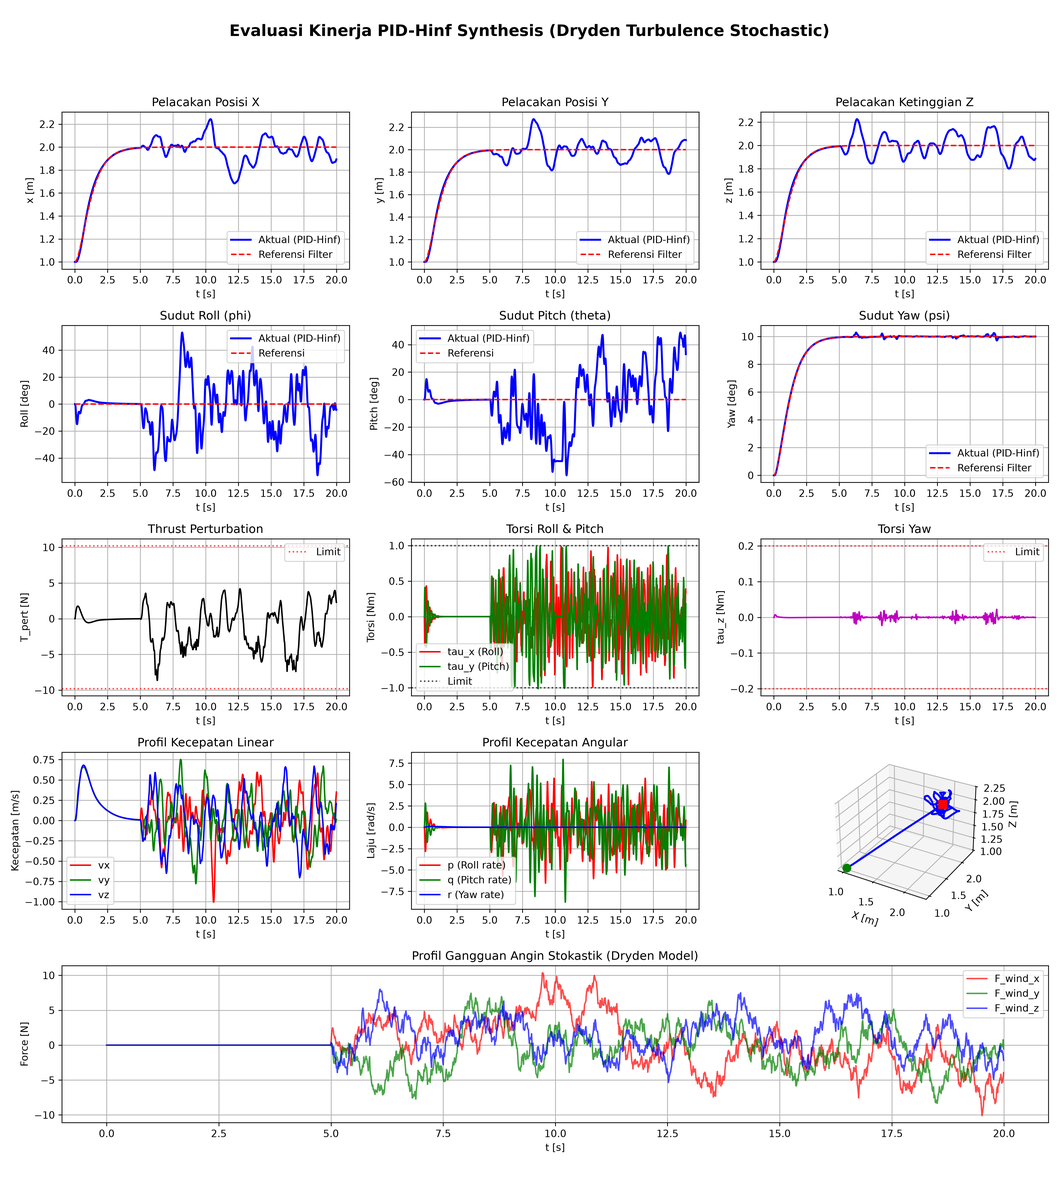
\includegraphics[width=\linewidth]{assets/fig/grafik_pid_hinf_wind_turbulence}}
    \end{column}
    \begin{column}{0.40\textwidth}
      \vskip2mm
      \begin{itemize}\bulletgap\small
        \item Offline plant simulation used while choosing $\gamma$
        \item \emph{Not} from the Gazebo campaign --- shown only to illustrate
              the design step
        \item Every number in the talk comes from the flown runs instead
      \end{itemize}
    \end{column}
  \end{columns}
\end{frame}

\begin{frame}{B3 \textperiodcentered{} A cylinder found in flight re-plans only the lanes still ahead}
  \begin{columns}[T,onlytextwidth]
    \begin{column}{0.60\textwidth}
      \videoposter{h6_obstacle_detour}{0.92\linewidth}
      \figcaption{rect, \hinf{} \textperiodcentered{} 20\,s around the closest
        static approach \textperiodcentered{} \videonote}
    \end{column}
    \begin{column}{0.36\textwidth}
      \vskip3mm
      \begin{itemize}\bulletgap
        \item LiDAR confirms a cylinder never seen before
        \item Lanes below the sweep line are left alone
        \item Until the re-plan, the QP alone keeps it clear
        \item Closest static approach: \ObssurfRectHinf\,m
      \end{itemize}
    \end{column}
  \end{columns}
  \note{Point at the arc in the RViz pane rather than the Gazebo pane.
        Re-planning finished lanes would sweep them twice.}
\end{frame}


\begin{frame}{B4 \textperiodcentered{} Gain synthesis and linear analysis in full}
  \centering\scriptsize
  \setlength{\tabcolsep}{4pt}\renewcommand{\arraystretch}{1.25}
  \begin{tabular}{llcccccc}
    \toprule
    \textbf{Design} & \textbf{Loop} & $K_p$ & $K_i$ & $K_d$ &
      $\|G\|_\infty$ (s\textsuperscript{2}) & $\omega_c$ (rad/s) & PM / GM \\
    \midrule
    \cL{\lqr}  & outer & \KoutkpLqr  & \KoutkiLqr  & \KoutkdLqr
               & \HnormLqr  & \WcLqr  & \PmLqr\textdegree{} / \GmLqr\,dB \\
               & inner & \KinkpLqr   & --          & \KinkdLqr
               &            &         &            \\[0.3ex]
    \cH{\hinf} & outer & \KoutkpHinf & \KoutkiHinf & \KoutkdHinf
               & \HnormHinf & \WcHinf & \PmHinf\textdegree{} / \GmHinf\,dB \\
               & inner & \KinkpHinf  & --          & \KinkdHinf
               &            &         &            \\
    \bottomrule
  \end{tabular}
  \vskip2.4ex
  \begin{columns}[T,onlytextwidth]\scriptsize
    \begin{column}{0.47\textwidth}
      Outer loops: $Q=\mathrm{diag}(0.08,\,0.35)$, $R=1$ for LQR;
      $\mathrm{diag}(0.10,\,0.40)$ for $H_\infty$.
    \end{column}
    \begin{column}{0.47\textwidth}
      Inner loops: $Q=\mathrm{diag}(6,\,0.6)$, $R=0.05$;
      $\gamma_{\min}=2.54$, used at $\gamma=3.30$.
    \end{column}
  \end{columns}
\end{frame}

\begin{frame}{B5 \textperiodcentered{} Upset events in full}
  \centering
  \figcard{\includegraphics[width=0.88\textwidth]{fig_events}}
  \figcaption{(a) contact leading to loss --- rect, \lqr, iris\_2
    \textperiodcentered{} (b) near-contact with recovery --- plus, both
    controllers, iris\_2}
\end{frame}

\begin{frame}{B6 \textperiodcentered{} The $H_\infty$ graze: a violent excursion that still recovered}
  \begin{columns}[T,onlytextwidth]
    \begin{column}{0.58\textwidth}
      \videoposter{h4_upset_plus_hinf}{\linewidth}
      \figcaption{Slowed \SlowHfour$\times$ relative to real time
        \textperiodcentered{} \videonote}
    \end{column}
    \begin{column}{0.38\textwidth}
      \vskip2mm
      \begin{itemize}\bulletgap\small
        \item Agent 2 grazes the central cylinder between lanes 4 and 5
        \item Tilt \UpPlusHinfTilt\textdegree, altitude to \UpPlusHinfZmin\,m,
              clearance \UpPlusHinfSurf\,m
        \item Recovered in about 3\,s
      \end{itemize}
    \end{column}
  \end{columns}
\end{frame}

\begin{frame}{B7 \textperiodcentered{} The same graze under LQR was milder}
  \begin{columns}[T,onlytextwidth]
    \begin{column}{0.58\textwidth}
      \videoposter{h5_upset_plus_lqr}{\linewidth}
      \figcaption{Slowed \SlowHfive$\times$ relative to real time
        \textperiodcentered{} \videonote}
    \end{column}
    \begin{column}{0.38\textwidth}
      \vskip2mm
      \begin{itemize}\bulletgap\small
        \item Peak tilt \UpPlusLqrTilt\textdegree{} against
              \UpPlusHinfTilt\textdegree{} for $H_\infty$
        \item Altitude held at \UpPlusLqrZmin\,m against \UpPlusHinfZmin\,m
        \item The two are not ordered on every metric
      \end{itemize}
    \end{column}
  \end{columns}
\end{frame}

\begin{frame}{B8 \textperiodcentered{} The second loss needs three helpers}
  \begin{columns}[T,onlytextwidth]
    \begin{column}{0.58\textwidth}
      \videoposter{h2_fault_kill2}{\linewidth}
      \figcaption{rect, \hinf{} \textperiodcentered{} 25\,s around the second
        kill \textperiodcentered{} \videonote}
    \end{column}
    \begin{column}{0.38\textwidth}
      \vskip2mm
      \begin{itemize}\bulletgap\small
        \item Agent 7 killed at 32\% coverage, agent 4 already gone
        \item The merged region is larger, so three helpers take it
        \item Helper groups across both losses: \HelpersRectHinf
      \end{itemize}
    \end{column}
  \end{columns}
\end{frame}

\begin{frame}{B9 \textperiodcentered{} Older data in this repository disagrees, and here is why}
  \begin{itemize}\bulletgap
    \item A 3 September 2026 sweep under \texttt{results/skema5/} shows eight FAIL runs
    \item Superseded configuration; only 10 of its 40 matrix rows ever ran
    \item Four benchmark figures were deleted in August 2026 after the tooling
          was found to synthesise telemetry when CSVs were missing
    \item Current reporting prints \texttt{n/a} and never substitutes a value
    \item Every number in this talk comes from the 11--12 September campaign
  \end{itemize}
\end{frame}

\begin{frame}{B10 \textperiodcentered{} All eight recordings are available here and published}
  \begin{columns}[T,onlytextwidth]
    \begin{column}{0.68\textwidth}
      \begin{itemize}\bulletgap\small
        \item \hinf{} --- rect \CovRectHinf\% \textperiodcentered{} L-shape
              \CovLshapeHinf\% \textperiodcentered{} U-shape \CovUshapeHinf\%
              \textperiodcentered{} plus \CovPlusHinf\%
        \item \lqr{} --- rect aborted \textperiodcentered{} L-shape
              \CovLshapeLqr\% \textperiodcentered{} U-shape \CovUshapeLqr\%
              \textperiodcentered{} plus \CovPlusLqr\%
        \item The next slides hold the full recordings --- jump to one if a
              specific region comes up
      \end{itemize}
    \end{column}
    \begin{column}{0.26\textwidth}
      \centering\playlistqr[22mm]\\[1ex]
      {\color{epicmuted}\scriptsize public playlist}
    \end{column}
  \end{columns}
\end{frame}

\begin{frame}{B11 \textperiodcentered{} Full mission --- rect, \lqr{} (aborted)}
  \centering\videoposter{rect_lqr}{0.62\textwidth}
  \figcaption{stopped at \TmisRectLqr\,s --- the full recording of the failure
    \textperiodcentered{} \videonote}
\end{frame}
\begin{frame}{B12 \textperiodcentered{} Full mission --- L-shape, \hinf}
  \centering\videoposter{l_shape_hinf}{0.62\textwidth}
  \figcaption{\CovLshapeHinf\% in \TmisLshapeHinf\,s \textperiodcentered{} \videonote}
\end{frame}
\begin{frame}{B13 \textperiodcentered{} Full mission --- L-shape, \lqr}
  \centering\videoposter{l_shape_lqr}{0.62\textwidth}
  \figcaption{\CovLshapeLqr\% in \TmisLshapeLqr\,s \textperiodcentered{} \videonote}
\end{frame}
\begin{frame}{B14 \textperiodcentered{} Full mission --- U-shape, \hinf}
  \centering\videoposter{u_shape_hinf}{0.62\textwidth}
  \figcaption{\CovUshapeHinf\% in \TmisUshapeHinf\,s \textperiodcentered{} \videonote}
\end{frame}
\begin{frame}{B15 \textperiodcentered{} Full mission --- U-shape, \lqr}
  \centering\videoposter{u_shape_lqr}{0.62\textwidth}
  \figcaption{\CovUshapeLqr\% in \TmisUshapeLqr\,s \textperiodcentered{} \videonote}
\end{frame}
\begin{frame}{B16 \textperiodcentered{} Full mission --- plus, \hinf}
  \centering\videoposter{plus_hinf}{0.62\textwidth}
  \figcaption{\CovPlusHinf\% in \TmisPlusHinf\,s \textperiodcentered{} \videonote}
\end{frame}
\begin{frame}{B17 \textperiodcentered{} Full mission --- plus, \lqr}
  \centering\videoposter{plus_lqr}{0.62\textwidth}
  \figcaption{\CovPlusLqr\% in \TmisPlusLqr\,s \textperiodcentered{} \videonote}
\end{frame}

\end{document}
